\chapter{\label{cha:translationese}Translation Detection}
This chapter establishes the premises of the investigated hypothesis that the amount of translationese manifested in a translation can be a good predictor of the level of professionalism and quality. 

Sections~\ref{sec:detect} and~\ref{sec:bestof} have the results of translationese classifications on professional and student translations to demonstrate that the selected hand-engineered features are, in fact, effective to capture translationese. 
To make sure that the proposed features are competitive in a translation detection task, their performance is contrasted with other representations including content-dependent features. 
If our hypothesis stands, we can expect that the more salient translationese indicators will also be good quality predictors. 
To shed more light on feature subsets and individual variables that can be considered most effective in capturing translationese, we analyse outcomes of automatic feature selection and perform univariate analysis for the three proposed types of features in Section~\ref{sec:bestof}.

The chapter opens with a description of the experimental setup for classification tasks including details on learning algorithms, generation of alternative representations and numeric data preprocessing (Section~\ref{sec:my_classifiers}).

\section{\label{sec:my_classifiers}Experimental Setup}

\paragraph{Dataset and proposed translationese indicators} The input to classifiers was arranged as a table of 3055 rows by 167 columns. In that table each row represented a document (including sentence-aligned source texts for parallel subcorpora). Columns stored three labels, six meta descriptors of each document-instance (document ID, language, word count, number of sentences, raw text and lemmatised text) and 158 hand-engineered numeric features from the attempted manual feature sets. 

The labels reflect three binary categories, listed below to introduce their shorthand names used throughout all experiments:

\begin{description}\compresslist{}
	\item[stu/pro vs ref:] categories in a translationese classification based on either (random) student or professional translations;
	\item[stu vs pro:] categories in a classification to capture professionalism (see Section~\ref{ssec:var} in Chapter~\ref{cha:pro_qua});
	\item[bad vs good:] categorial document-level quality labels from holistic assessment of student translations verified in a separate annotation effort (results on this dataset appear in Section~\ref{ssec:bin}).
\end{description}

In tabled results below linguistically-motivated translationese-aware feature sets are represented as follows:
\begin{description}\compresslist{}
	\item[UD:] 60 features extracted from Universal Dependencies annotations (see Section~\ref{ssec:ud});
	\item[collgram:] 24 features representing abstract collocational properties of texts (see Section~\ref{ssec:coll});
	\item[ngram:] 10 features from 1-2-3-gram frequency lists and from n-gram-based language models (see Section~\ref{ssec:ngram});
	\item[all:] combination of the above feature sets (94 features).
\end{description}  

Adding actual raw and lemmatised texts into the table and setting the random seed helped to ensure that the same instances were found in the same order in the same folds regardless of the representation used: manual features or vectors from pre-trained embedding models.

\paragraph{\label{pg:vectors}Alternative document representations} To demonstrate the competitiveness of hand-engineered features, we compare them with a number of alternative representations. 

The chance-level baseline is calculated using a stratified strategy, which ignores the input features altogether. Its predictions are based on randomly assigned class value to each feature in a row respecting the class distribution in the training data.

The hand-engineered features are all relatively content-independent. We compare their performance to surface-feature-based \gls{tf-idf} representation and to text vectors generated by mean-pooling of embeddings from several Transformer models. 
The vectorisation setup in each case was implemented as follows.
\label{pg:tfidf_meth}
\textit{Tf-idf} is a numeric representation for documents which uses weighted frequencies of a corpus vocabulary items as vector components. Those vectors were calculated using a dedicated \textit{scikit-learn} utility. We used all available documents in the Russian language as the underlying corpus. 
To reduce vocabulary size and increase informativity of this representation, the corpus was lemmatised. All proper names and their sequences were replaced with a \textit{PROPN} tag (e.g \textcyrillic{\textit{говорит Максимилиан Чуперски}} [says Maksymilian Czuperski] --> \textcyrillic{\textit{говорить PROPN}}). All digits were replaced with \textit{X} (e.g. \textit{12 октября 1982; 2,5;  1980-е} --> \textit{XX October XXXX; X.X; XXXXs}). The vocabulary was built to include word unigrams, bigrams and trigrams. The vector size was limited to 5000 most frequent corpus vocabulary items. Other hyper-parameters were set to the default values from the library. 
% we should have excluded items in English as simple give-aways for translations vs non-translations, because translatons often retain the proper names in the SL in parenthesis, and those were not tagged as PROPN but as foreign_word.

We also used four pre-trained contextualised embedding models to infer vectors for documents in our experiments. These models aim to generate distributed representations of document meaning (in a broad sense) and are content-dependent. The models are open-source and freely available from the \textit{HuggingFace} repository.

We selected the models that were trained to solve various NLP tasks deemed more suitable for our purposes. The list below gives a brief description of each model. 
\begin{description}\compresslist{}
	\item[stsb-xlm-r-m:] a multilingual model\wlvfootnote{\url{huggingface.co/sentence-transformers/stsb-xlm-r-multilingual}} trained using Sentence-BERT (SBERT), a~\gls{SOTA} framework to compute sentence representation~\cite{Reimers2019}. SBERT is a generic name for contextualised embedding models fine-tuned on various sentence-level tasks such as question-answering, sentiment, paraphrasing, etc. The model we used was a multilingual XLM-R fine-tuned on \gls{STS} task;
	
	\item[TQmono-m:] a cross-lingual model for many languages\wlvfootnote{\url{TransQuest/monotransquest-da-multilingual}} trained by the more successful architecture from \textit{TransQuest} package~\cite{Ranasinghe2020}, to solve MT quality estimation task based on DA scores;
	% these models generate word embeddings that are mean-pooled under the hood by SentenceTransformers library 
	
	\item[ruRoberta:] a dedicated Russian model\wlvfootnote{\url{huggingface.co/sberbank-ai/ruRoberta-large}} trained as a full-mask language model using \textit{RoBERTa}, an optimised BERT transformers training method proposed by~\cite{Liu2019};
	
	\item[mdeberta3:] a multilingual version of \textit{DeBERTa}~\cite{He2021}, an improvement on \textit{BERT} and~\textit{RoBERTa} word embedding architectures, trained on 2.5T CommonCrawl corpus for 100 languages \wlvfootnote{\url{huggingface.co/microsoft/mdeberta-v3-base}}. At the time of writing, it is \gls{SOTA} in word-level representation learning. 
\end{description}

The first two models generate sentence embeddings, while the last two output word embeddings, which were averaged to get sentence embeddings. Further on, the sentence embeddings were mean-pooled to obtain document vectors. 
Note that in most experiments we might not have enough datapoints to train these representations further on the labels available in our tasks in a fine-tuning setup. % Methodologically, we use transfer learning approach? 
%768-dimensional vector

For all experiments and representations, the input data was transformed with \textit{scikit-learn Standard Scaler}. This function standardises the values of each feature column-wise (i.e. independently) to have zero mean and unit variance of 1. It helps to put all features on the same scale regardless of the original measurement unit, and avoid the situation when features with large variance dominate the learning process overshadowing the differences on other features.

\paragraph{Algorithms} Both classification and regression experiments (reported in Chapter~\ref{cha:pro_qua}) are based on \gls{SVM} algorithm as implemented in \textit{scikit-learn}, a Python library for machine learning. 
This algorithm was shown to be superior to tested alternatives for translationese classification in a number of research projects (see, for example,~\cite{Ilisei2010}). It is also known to be robust to high-dimensional datasets where the number of instances is similar or even smaller than the number of features.

This research is focused on testing the hypothesis whether translationese indicators are good predictors of translation quality, and on exploring the relations between a number of diverse representations and quality labels. Our aims did not include achieving the best performance possible for given datasets, therefore, we do not report results for various SVM kernels and other parameters of algorithms that can be discovered through optimisation studies. 
Instead, the classification experiments are based on a linear kernel SVM and regularisation parameter $C=1.0$ (default for SVM \textit{scikit-learn} setting).

SVM uses pairwise distances between the datapoints from given categories and identifies instances with most similar vectors (called \textit{support vectors}). Then, it calculates a maximum hyperplane separating these support vectors, by assigning positive or negative weights to features to put instances on the required side of the hyperplane and reduce algorithm error. Instances that are found on the opposite sides of the hyperplane are assigned to the respective categories. 
\textit{C} parameter is the cost of misclassification, or tolerance for errors. Higher \textit{C} values lead to fewer errors in the training set, and to a more overfit model, which would not generalise well. It will result in poorer performance on a test set.

Although the datasets in our experiments are reasonably well-balanced we kept the \textit{class\_weight} parameter of the algorithm set to \textit{balanced}. 

As a sanity check, we implemented a simple sequential neural model to replicate the performance of SVM-based classifiers on exactly the same inputs. The neural model~\label{pg:neural} was designed using \textit{Keras} \gls{API} integrated into \textit{TensorFlow 2.0} (tf.keras). It is promoted as the standard interface for deep learning.\wlvfootnote{Both \textit{TensorFlow} (\url{github.com/tensorflow/tensorflow}) and \textit{Keras} (\url{keras.io/}) are open-source libraries for deep learning with Python.}  

The neural model used document vectors as input and was compiled with two dense (i.e. fully-connected) hidden layers. The first layer was  made of 16 neurons and was activated with \gls{ReLU} function, which output zero for negative input values and returned the input directly if the input was positive. 

The output layer for the classification task was activated with a \textit{sigmoid} function, which mapped all inputs in the real number domain into the range of 0 to 1. It transformed input values that were much larger than 1.0 to 1.0, values much smaller than 0.0 were snapped to 0.0. In fact, this layer output the probability of a test instance belonging to a positive class. The threshold of 0.5 was used to obtain the model predictions of binary categories. 

%For the regression task, we use \textit{linear} activation function, which scales each input by a learnt factor and assumes linear relation between inputs and targets. 

% mean absolute error can be used as loss function for regression
The model was compiled with \textit{binary cross-entropy} as loss function for the classification tasks. \textit{Adam optimiser} was used for gradient descent calculations; each experiment was set to run for 10 epochs with batch size 8.

We also monitored the learning process with an \textit{EarlyStopping} class. It was set to keep track of accuracy across 10 training epochs for each run of the experiment. The training stopped if the gain in the algorithm performance was less than 0.0001 for three consecutive epochs. 

Another standard ML setting which prevents over-fitting, especially with high-dimensional data, is cross-validation. 
The data was split 10 times into a training and test sets in a cycle, respecting the balance of categories, so that each instance appeared in a test set at least once. We report the averaged results (and their standard deviation) across 10 runs (folds) of each experiment. All scores are expressed as percentages. 

We use the standard evaluation metrics for classification problems as described in Section~\ref{ssec:task} (page~\pageref{pg:eval_setup}). 

\paragraph{Feature Analysis Methods}
% correlation matrix for feature selection and analysis: https://medium.com/geekculture/feature-selection-in-machine-learning-correlation-matrix-univariate-testing-rfecv-1186168fac12
Detection of the best translationese indicators is performed using \gls{RFE} technique. 
We believe that some features might form functional subsets that would perform better together. \gls{RFECV} method was used to retrieve a dynamic set of most informative features for each dataset. 
\gls{RFECV} applies an algorithm (a linear SVM in our case) to a feature space reduced by one feature with the least importance for each subsequent run of the experiment. The importance of features is established using weights assigned by the algorithm. The process is continued to obtain the best performance across several cross-validation folds (five, in our case). We scaled each features before selection to have zero mean and variance of 1. 

We also used weights (and their visualisations) assigned by linear-kernel SVM in univariate feature analysis. According to explanations in~\citet{Volansky2015}, high feature weights are a good indication of a significant difference between the two classes, but lower feature weights might not mean lack of discriminative power because feature weights can be reduced taking into account possible inter-dependencies among features in the feature set.  

Apart from providing information about the more salient linguistic properties of each text category, feature selection allows to reduce the feature space by removing noisy features (if any), which might lead to an increase in the algorithms performance.
%Feature selection is applied to the most effective hand-engineered (interpretable) feature sets only.

To establish major trends in translational behaviours that could be associated with the observed properties of each translation categories, we developed a sequence of statistical univariate tests that describe the  differences between each pair of categories involved in a translationese study (source texts, translations and non-translated TL reference).

Non-parametric statistical tests were selected in all cases, because the values of most features were not normally distributed for either of the document categories. For example, here were only 12 features in non-translated subcorpus (out of 94 total) where the null hypothesis of normal distribution was not rejected based on \textit{Shapiro-Wilk test}, a statistic test of normality.
For many manual features, the compared categories of documents also had unequal variances.   
\textit{Bartlett statistic}, which tests for homogeneity of variances across two samples, revealed that there were 68 feature with unequal variances in the translationese classification experiment based on professional translations, for example. 

These peculiarities in the distributional properties of features also explain the choice of \textit{RFE} algorithm over \textit{ANOVA} for feature selection. The latter compares between-categories and within-categories variation, and assumes normal distribution and equal variances between samples.

Statistical significance was tested using \textit{two-tailed Mann-Whitney U Test for independent samples} and \textit{Wilcoxon signed-rank test for paired samples} as a non-parametric alternative for data that violates the assumption of normal distribution made by Student's t-test.

Additionally, we measured the strength of the relationship between each variable (feature) and target labels using 5-fold cross-validated \textit{Logistic regression} which returned macro F1-scores in the classification setup. 
% we cannot use Spearman with 0, 1 labels as it relies on differences in ranks
The choice of the method is explained as follows. In many of our experiments we had to estimate the association between continuous and binary categorical variables, and could not use either \textit{Cohen's D} effect size metric or regular correlation coefficients, because it is impossible to calculate the covariance in this setup. The use of a classifier as an association metric builds on an assumption that if we can accurately predict a categorical variable from a continuous variable, they can be considered correlated. 

We also used scatter plots and line plots to present the results of \gls{PCA} for some of our representations. By analysing covariances between features, PCA attempts to reduce multidimensional data to a few new features that aggregate maximum information of the original representation. Although dimensionality reduction simplifies the relations between datapoints, it can be useful to visually study how well each representation captures the distinction between categories. 

All examples, unless indicated otherwise are taken from student translations. In the tables, we highlighted the best results for manually engineered feature sets and boxed the best results for content-dependent classifiers. The best results are defined as the results that were not significantly outperformed by any other model in that category at the confidence level of 0.05. 

\section{\label{sec:detect}Translationese Classifications}

This section presents the results of translationese classifications on professional and student translations. The quality of these classifications indicates how well a given feature set or representation can distinguish translations from non-translations. \citet{Hu2021} raises a question about the level of accuracy that is high enough to accept a feature or a feature set as discriminative for the categories at hand. To give an idea of what performance is achievable, we report results from the best-performing content-dependent classifier in our experimental setup, namely, \textit{mdeberta3}.
 
Statistical tests showed that there were no statistically significant differences between the performance on \textit{mdeberta3} vectors, on \textit{ruRoberta-large} and on \textit{tf-idf} representation. For considerations of space, we omit the results on these models from the tables below.

Tables~\ref{tab:pro-ref} and~\ref{tab:stu-ref} aggregate results for a linear SVM classifier on three distinct hand-crafted delexicalised feature sets and their concatenation (\textit{all}) for professional and students translations, respectively. They are put into perspective of chance level and contextualised embeddings results. Note that most of translationese indicators proposed by~\citet{Volansky2015} (and used as a baseline in some translationese research) were implemented in this study and included in either \textit{UD}, \textit{collgram} or \textit{ngram} feature sets.  

Results for a neural classifier (page~\pageref{pg:neural}), which was run in the same settings as an alternative for a linear SVM, appear in Appendix~\ref{appx:neural_res}. Systematic comparison between the SVM and neural classifier showed that out of 40 settings across various feature sets in four binary classifications, statistically significant differences between the algorithms were observed in only four cases (as measured with a two-sided t-test using F1-scores from 10 cross-validation folds, at confidence level $\alpha=0.05$). It confirms that in terms of learnability, we achieved a reasonable performance level. 

Generally, both translation varieties were easily separable from originally-authored texts on all attempted representations. Both lowest and highest F1-scores were seen on student translations: 65.63\% on \textit{collgram} feature set and 98.36\% on \textit{mdeberta3} vectors. 

Structural morphosyntactic classifiers (UD) with linear SVM kernel demonstrated competitive performance and returned macro F1-score of 90.22\% and 88.96\% for professional and student translations, respectively.

\begin{table}[H]
	\centering
	\begin{tabular}{p{2.9cm}|llll}
		\toprule
		& Accuracy        & Precision       & Recall        & F1              \\
		\midrule
		chance          & 47.72 (+/-5.93) & 47.72 (+/-5.93) & 47.70 (+/-6.00) & 47.58 (+/-5.95) \\
		\midrule
		UD              & 90.34 (+/-2.73) & 90.51 (+/-2.59) & 90.32 (+/-2.98) & 90.22 (+/-2.81) \\
		collgram        & 70.82 (+/-5.11) & 71.15 (+/-5.09) & 71.16 (+/-5.07) & 70.71 (+/-5.08) \\
		ngram           & 86.12 (+/-2.96) & 86.07 (+/-3.04) & 86.30 (+/-3.07) & 86.04 (+/-2.99) \\
		all             & 92.45 (+/-2.72) & 92.41 (+/-2.73) & 92.53 (+/-2.81) & \textbf{92.38} (+/-2.76) \\
		%		\hline
		%		tfidf           & 96.89 (+/-1.91) & 96.97 (+/-1.98) & 96.81 (+/-1.90) & 96.85 (+/-1.93) \\
		%		\hline
		%stsb-xlm-r-m   & 94.56 (+/-1.68) & 94.69 (+/-1.74) & 94.38 (+/-1.69) & 94.49 (+/-1.70) \\
		%TQmono-m & 95.45 (+/-2.07) & 95.42 (+/-2.14) & 95.49 (+/-2.02) & 95.41 (+/-2.09) \\
		%		ruRoberta & 95.56 (+/-2.05) & 95.52 (+/-2.11) & 95.54 (+/-2.02) & 95.51 (+/-2.07) \\
		\midrule
		mdeberta3  & 96.67 (+/-1.65) & 96.74 (+/-1.63) & 96.64 (+/-1.64) & \boxit{0.4in} 96.63 (+/-1.66)\\		
		\bottomrule
	\end{tabular}
	\caption{\label{tab:pro-ref}Professionals: translationese classification. Support: N(pro)=404, N(ref)=497}
\end{table}

The superior performance of content-dependent classifiers on this task is expected, because translations and non-translations can be on different topics. Classifiers that exploit lexical (string) features are likely to capture less interesting topical distinctions between the corpora.

\begin{table}[H]
	\begin{tabular}{l|llll}
		\toprule
		representation    & Accuracy        & Precision       & Recall          & F1              \\
		\midrule
		chance          & 50.05 (+/-3.72) & 48.65 (+/-3.80) & 48.62 (+/-3.88) & 48.59 (+/-3.84) \\
		\hline
		UD              & 89.41 (+/-4.25) & 89.20 (+/-4.28) & 88.93 (+/-4.57) & 88.96 (+/-4.46) \\
		collgram        & 67.50 (+/-6.58) & 66.64 (+/-6.93) & 65.54 (+/-6.22) & 65.63 (+/-6.40) \\
		ngram           & 86.40 (+/-3.29) & 86.30 (+/-3.18) & 85.27 (+/-3.99) & 85.61 (+/-3.70) \\
		all             & 92.30 (+/-2.03) & 92.25 (+/-2.20) & 91.81 (+/-2.18) & \textbf{91.96} (+/-2.10) \\
		%		tfidf           & 98.07 (+/-1.34) & 98.04 (+/-1.46) & 97.99 (+/-1.39) & 98.00 (+/-1.40) \\
%		stsb-xlm-r-m   & 90.49 (+/-3.06) & 90.96 (+/-3.26) & 89.46 (+/-3.23) & 89.96 (+/-3.19) \\
%		TQmono-m & 94.11 (+/-2.48) & 94.30 (+/-2.52) & 93.52 (+/-2.68) & 93.82 (+/-2.61) \\
		%		ruRoberta & 97.83 (+/-1.40) & 97.96 (+/-1.34) & 97.60 (+/-1.65) & 97.73 (+/-1.48) \\
		\midrule
		mdeberta3  & 98.44 (+/-1.43) & 98.64 (+/-1.33) & 98.16 (+/-1.64) & \boxit{0.4in} 98.36 (+/-1.49)\\
		\bottomrule
	\end{tabular}
	\caption{\label{tab:stu-ref}Students: results of translationese classification. Support: N(stu)=334, N(ref)=497}
\end{table}

For both translation varieties, structural UD features, which were focused in this study, significantly outperformed the other two manually-constructed feature sets. The results on 10 features from n-gram language models were 3-4\% lower, while collocational features were 19-23\% worse. 

\textit{Collgram} feature set, designed to capture collocational peculiarities of translational language, returned the lowest performance (still much above the stratified random baseline). It also demonstrated higher volatility across the folds, with standard deviations as high as 5 and 6\%. The performance of SVM classifier on UD features was more stable, especially for professional translations, where STD averaged at around 2.8. 

\textit{Collgram} and \textit{n-gram} features did not yield any real gain in classifier performance, when combined with UD feature set. Although F1-score on \textit{all} features was a 2\% higher for both classifications, the difference was not statistically significant (at $\alpha=0.05$ confidence level).

%Interestingly, the neural classifier returned much lower results than SVM on 10-dimensional n-gram vectors, especially for professional translations, where F1-score went down from 86.04 (SVM) to 69.02\% for neural classifier (see Appendix~\ref{appx:neural_res} for all neural classifier results). 
% ratio of highly- and negatively-associated collgrams, ratio of all detected collgrams, average association score

\paragraph{Performance of translationese classifiers on two translation varieties}
Overall, the quality of translationese classifications for professional and student translations was approximately the same in most setups. This observation runs contrary to our expectations. We expected student translations to be less fluent and less similar to non-translations and, therefore, easier to detect. 
It is even more surprising that professional translations should return slightly higher classification results than student translations, particularly on UD features (F1-score 90.22\% vs 88.96\% for professionals and students by SVM, 90.43\% vs 90.1\% by neural classifier).

Although it is not a common practice, \citet{Demvsar2006} argues that non-parametric \textit{Mann-Whitney U rank test} (aka Wilcoxon rank sum test) on two independent samples can be used to compare performance of one algorithm over multiple datasets. 
According to this test, there was no evidence that professional translations were more distinct from non-translations than students (at 0.05 confidence level) for either SVM or neural classifier on any representation (except \textit{stsb-xlm-r-m} on both SVM and neural classifier).
Based on the difference observed on \textit{stsb-xlm-r-m}, we can conclude that professional translations were semantically less similar to the reference subcorpus than texts translated by students. 

To visually explore the relations between text categories in the two experiments, we cast multidimensional document vectors into a 2D space using PCA. 
The scatter plot in the left-hand panel of Figure~\ref{fig:vars-ud} presents non-translations, student and professional translations along with their sources using the first two principal components, constructed by PCA from UD vectors.

\begin{figure}[H]
	\begin{minipage}[c]{0.5\linewidth}
		\centering
		2D representation of document types
		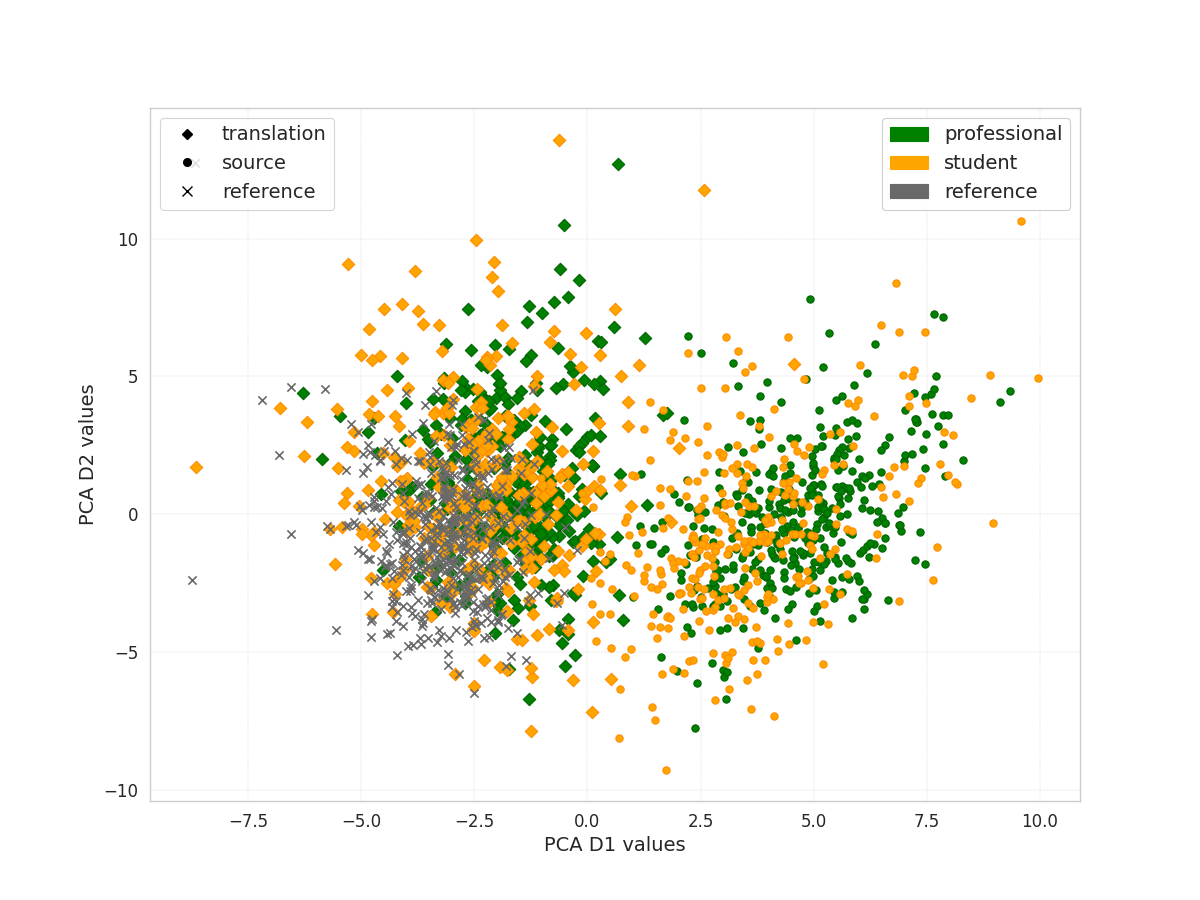
\includegraphics[width=\linewidth]{figures/pca/src-var-ttype-ud-PCA-scatter}
	\end{minipage}	
	\begin{minipage}[c]{0.5\linewidth}
		\centering
		Distribution along PCA D1
		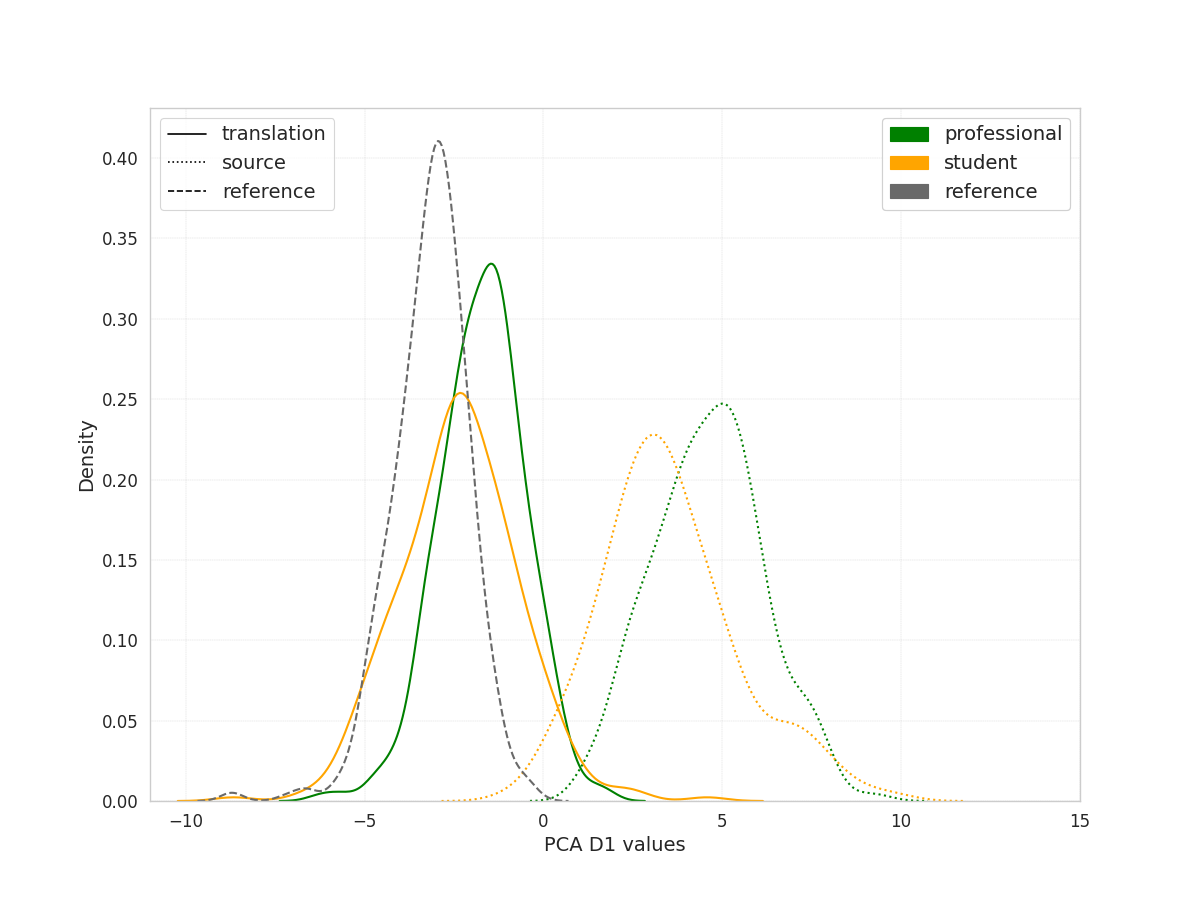
\includegraphics[width=\linewidth]{figures/pca/src-var-ttype-ud-PCA-D1-lines}
	\end{minipage}
	\caption{\label{fig:vars-ud}Visualisations of PCA transform based on \textit{UD} features}	
\end{figure}
  
Each marker represents a document from the respective colour-coded category. Coloured diamonds are used for translations, dots for source texts in English and dark grey crosses are non-translations in the TL. 
The most obvious distinction is between the two languages: Russian is on the left, English is on the right. 
It can be seen that all translations are shifted away from non-translations to the left towards source texts. 
The translation varieties are not clearly separated from non-translations and from each other. It means that the signal captured by fairly successful translationese classifications is distributed among the UD features and cannot be easily summarised by just two dimensions.
To be fair, PCA offers a very crude simplification for the underlying datasets. PCA D1 shown in Figure~\ref{fig:vars-ud} explains only 21\% of the total multivariate variability in the full UD dataset, with further 13\% captured on D2. 

Importantly, we can see a difference in location between English source texts for professional and student translations: green dots of professional translation sources in left-hand panel in Figure~\ref{fig:vars-ud} seem to be further away to the right from the centre of the plot. ST is a known factor in shaping the properties of translations, and this difference should be taken into consideration in feature analysis. 

It can be argued that student translations (shown in orange) are the least compact cloud without a distinct location, while professional translations are a bit more homogeneous. This observation is supported by a more focused representation of document values on x-axis (PCA D1) in the right-hand panel using a kernel density estimation plot (a smoothened and scaled version of a histogram plot). The group of three line plots on the left shows the variation in distributions of PCA D1 values across the document classes in Russian. The shape of the flatter orange solid-line curve for student translations suggest more variability in the data. Both student and professional translations are shifted to the right from non-translations (grey dashed line) towards the area of English sources. We can tentatively conclude that D1 captures language-contrast-related properties of documents.
% UD Variance explained per dimension (if lose_src=False):  [0.21163434 0.13134273]
% UD Variance explained per dimension (if lose_src=True):  [0.16399743 0.13674201]

By way of comparison, consider the same types of visualisations for our best performing representation, namely for \textit{mdeberta3}, in Figure~\ref{fig:vars-deberta}. 

\begin{figure}[H]
	\begin{minipage}[c]{0.31\linewidth}
		\centering
		PCA	2D 
		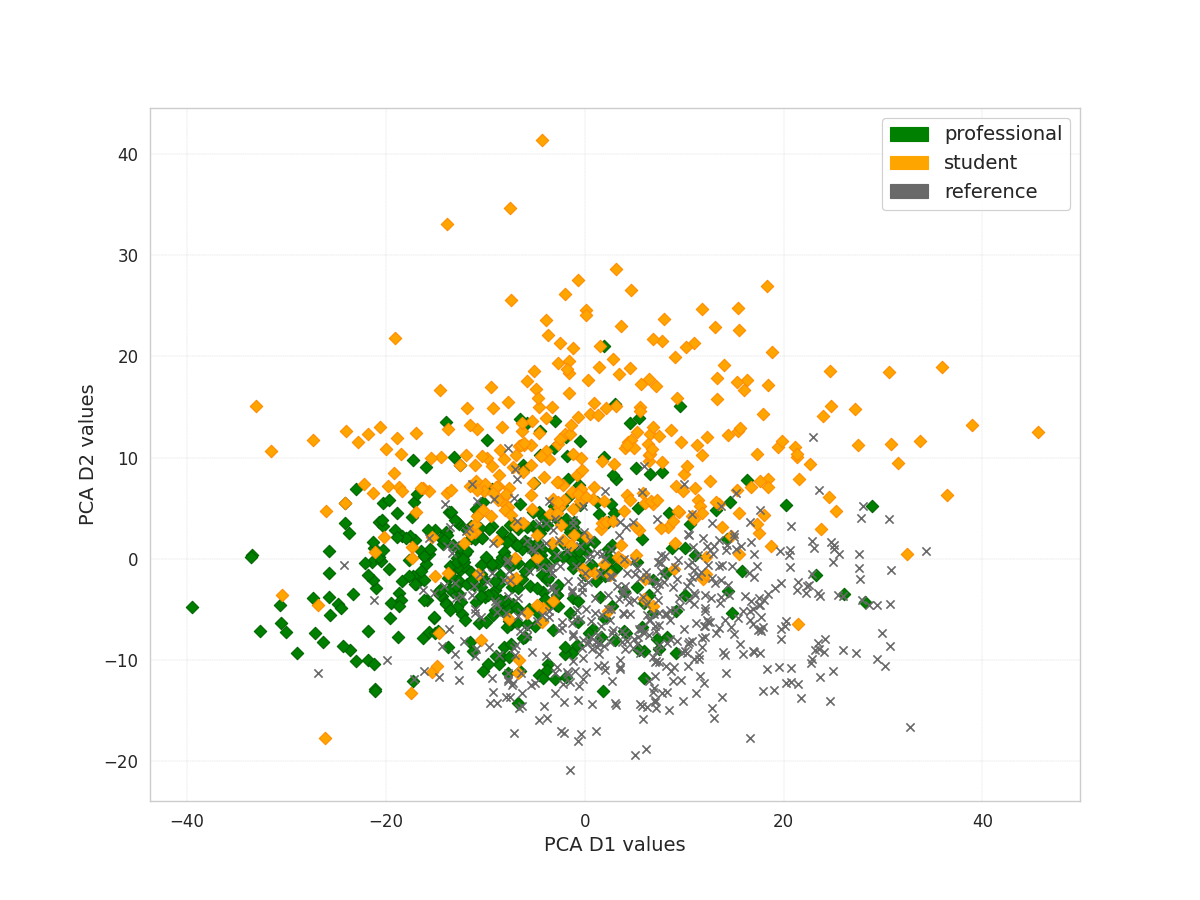
\includegraphics[width=\linewidth]{figures/pca/var-ttype-mdeberta3-base-PCA-scatter}
	\end{minipage}	
	\begin{minipage}[c]{0.31\linewidth}
		\centering
		PCA D1
		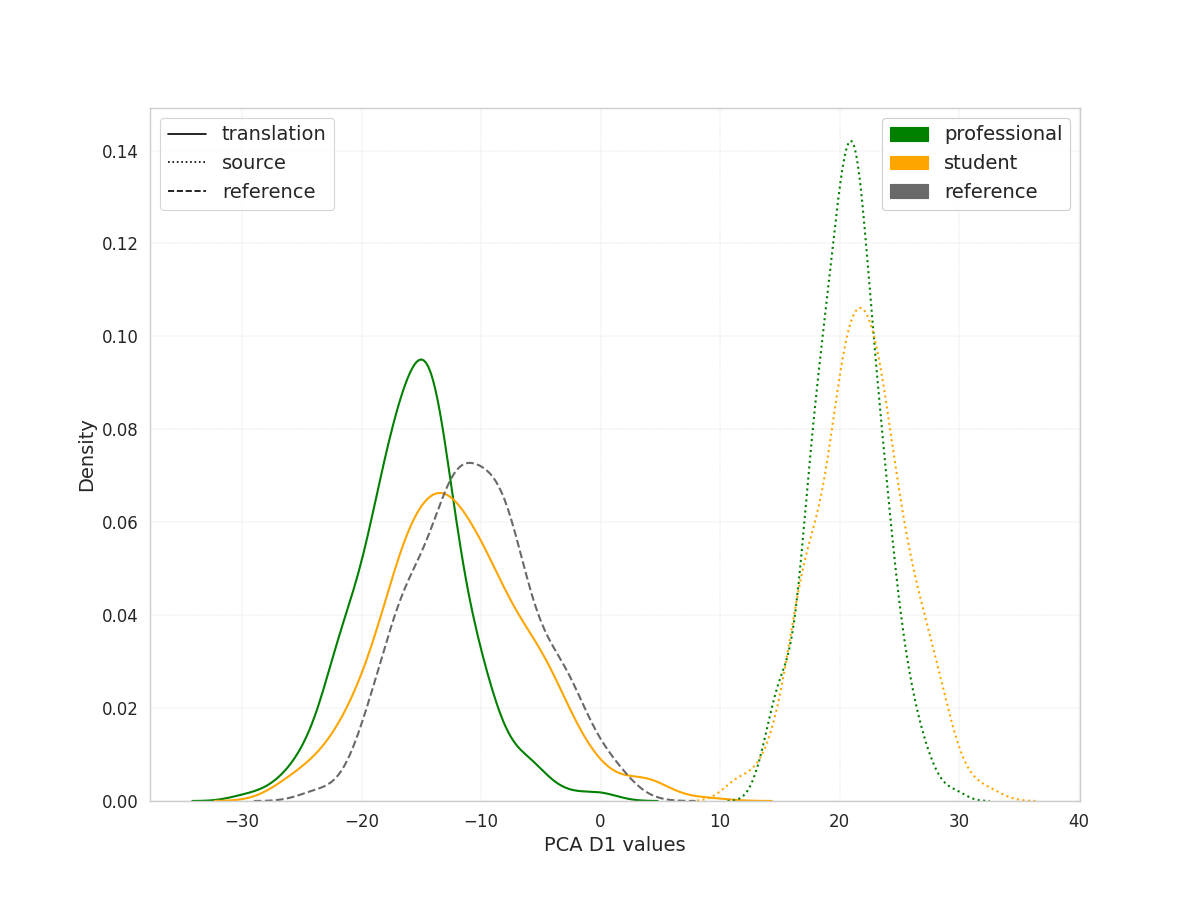
\includegraphics[width=\linewidth]{figures/pca/src-var-ttype-mdeberta3-base-PCA-D1-lines}
	\end{minipage}
	\begin{minipage}[c]{0.31\linewidth}
		\centering
		PCA D2
		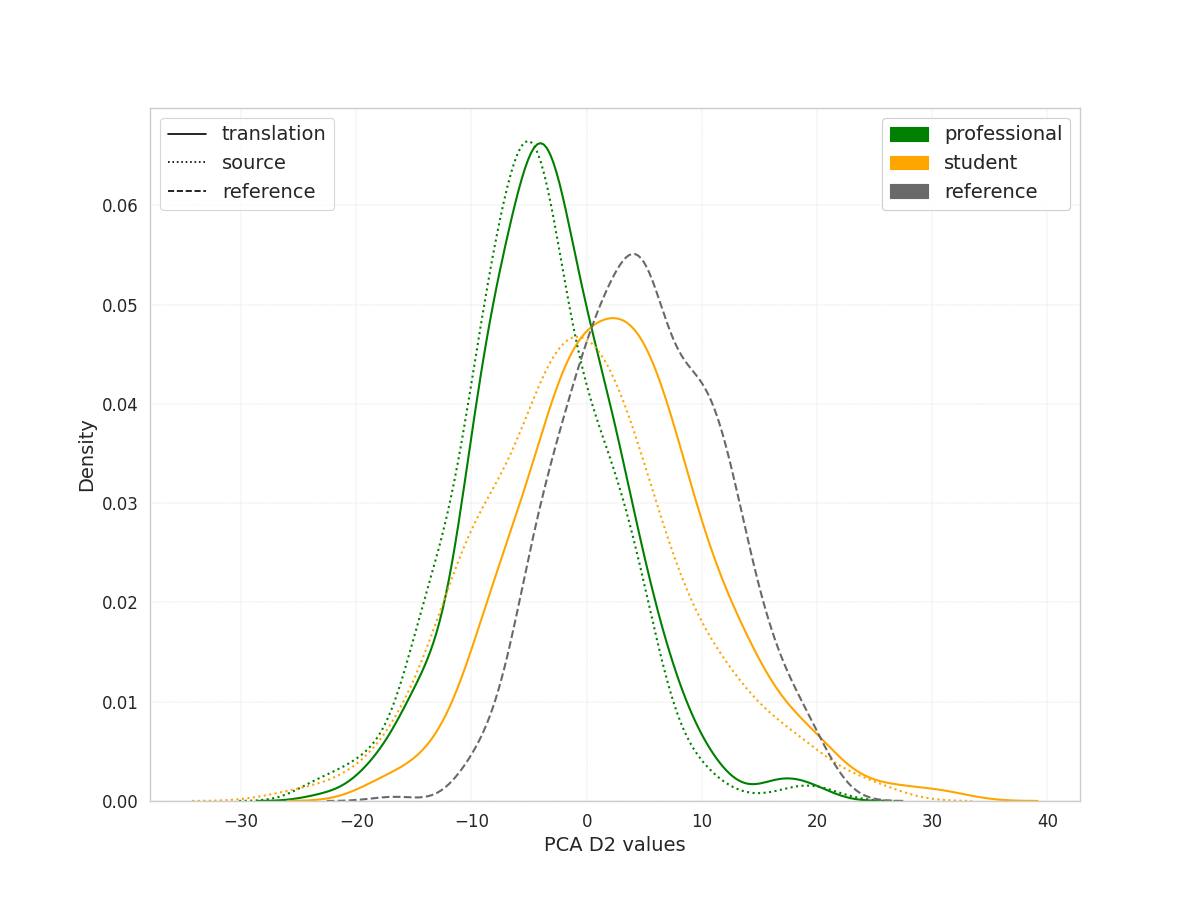
\includegraphics[width=\linewidth]{figures/pca/src-var-ttype-mdeberta3-base-PCA-D2-lines}
	\end{minipage}
	\caption{\label{fig:vars-deberta}Visualisations of PCA transform based on \textit{mdeberta3} representation}	
\end{figure}

If we exclude English sources from PCA analysis (they overshadow all other distinctions on multilingual vectors), the three classes of documents in the TL are more or less distinct and are located in different parts of the 2D scatter plot. D1 (x-axis) seems to capture the differences between professional translations and non-translations, while D2 (y-axis) values separate student translations from the other two categories. Unlike the previous representation, translations (regardless of professionalism level) were not grouped together against non-translations. If anything, student translations appear to have more in common with non-translations than with professional translations. It means that \textit{mdeberta3} did not really capture the commonalities of translations as an ontological text category. It is likely that the co-varying components of \textit{mdeberta3} vectors, aggregated by PCA, reflect semantic (topical) differences between categories along each of the axes. The right-most panel in Figure~\ref{fig:vars-deberta} suggests that student translation source texts are indeed semantically more similar to Russian non-translations than English source texts of professional translations. 
% mdeberta3 Variance explained per dimension (if lose_src=False):  [0.38012075 0.08784468]
% mdeberta3 Variance explained per dimension (if lose_src=True):  [0.21136208 0.09629121]

This impression is reproduced on \textit{stsb-xlm-r-m} vectors\wlvfootnote{\textit{Stsb-xlm-r-m} is a cross-lingual language model for many languages specifically trained to capture semantic similarities between sentences.} (see left-most panel in Figure~\ref{fig:other}). 
However, vectors from \textit{TQmono-m}, a Sentence Transformer fine-tuned on MT quality estimation task, when squeezed into one component by PCA, revealed the commonality between the two translation collections. Both demonstrate a shift away from non-translations (in either language). Interestingly, student translations are located further away from non-translated reference than professional translations, capturing the anticipated difference in the amount of translationese (see central panel in Figure~\ref{fig:other}). 
Finally, the right-most scatter plot in Figure~\ref{fig:other} shows that a dedicated Russian contextualised word embedding model also detects translationese per se (and not the confounding topical differences between text categories): it separates all translations from non-translations, but this distinction is captured on a weaker D2 component (y-axis), while D1 probably captures the variation in topical content.   

\begin{figure}[H]
	\begin{minipage}[c]{0.31\linewidth}
	\centering
	stsb-xlm-r-m PCA D1 
	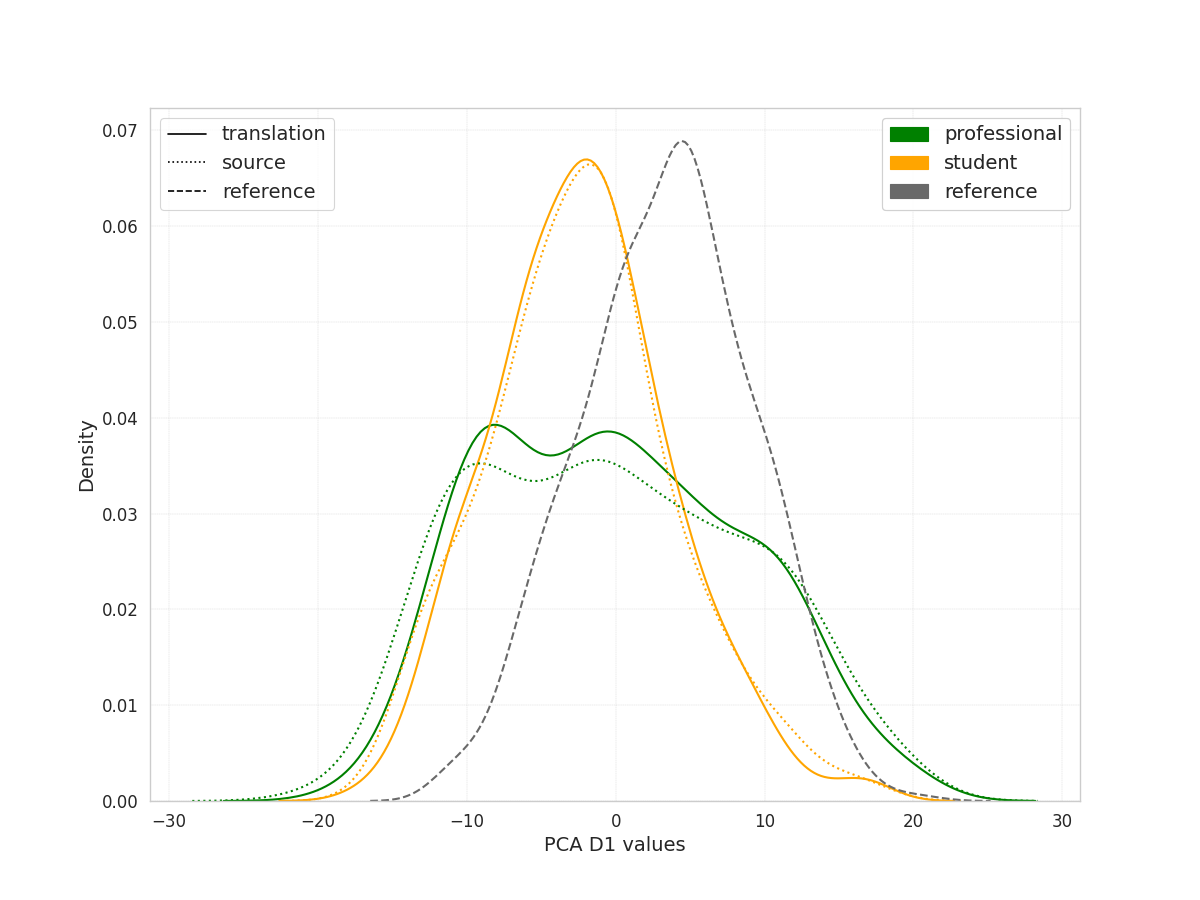
\includegraphics[width=\linewidth]{figures/pca/src-var-ttype-mXLM-R-PCA-D1-lines}
\end{minipage}	
\begin{minipage}[c]{0.31\linewidth}
	\centering
	TQmono-m PCA D1
	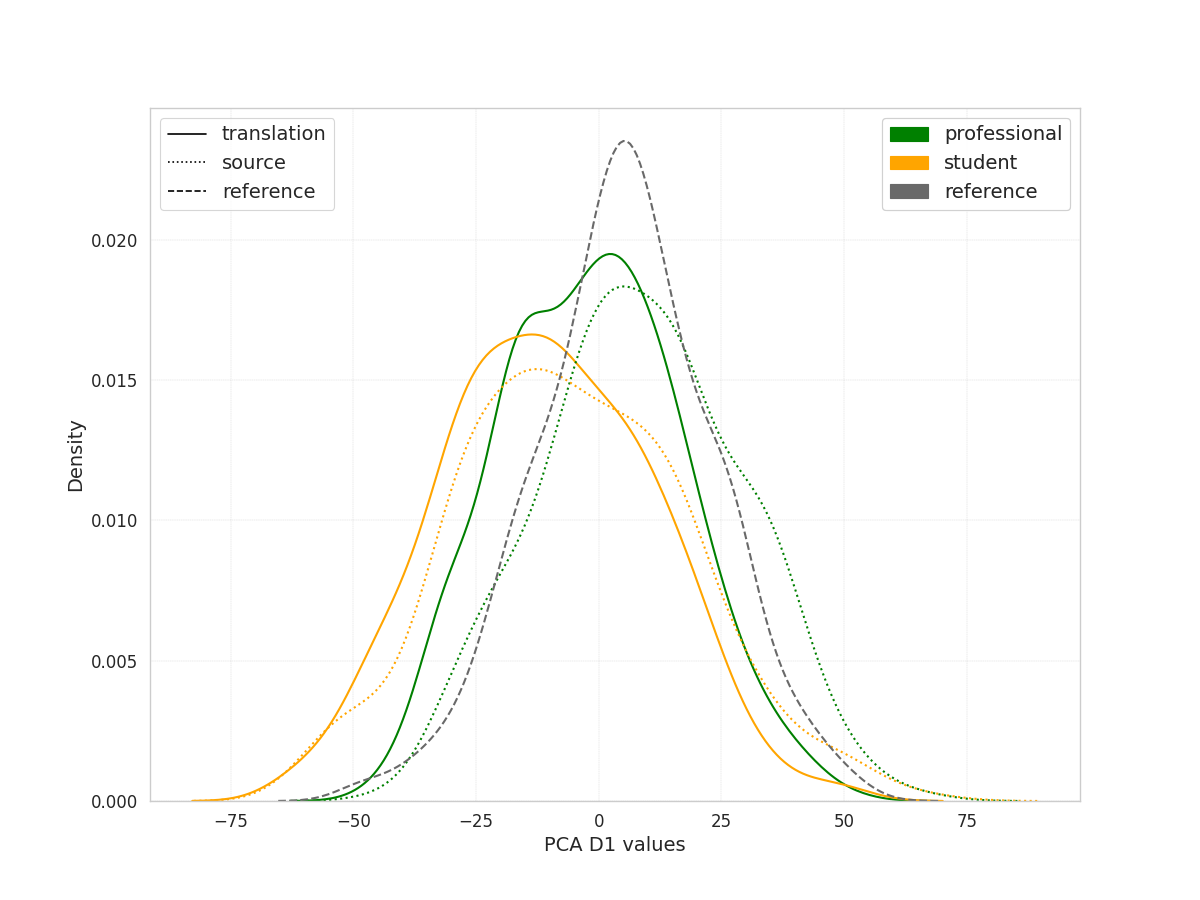
\includegraphics[width=\linewidth]{figures/pca/src-var-ttype-TQmono-m-PCA-D1-lines}
\end{minipage}
\begin{minipage}[c]{0.31\linewidth}
	\centering
	ruRoberta PCA 2D
	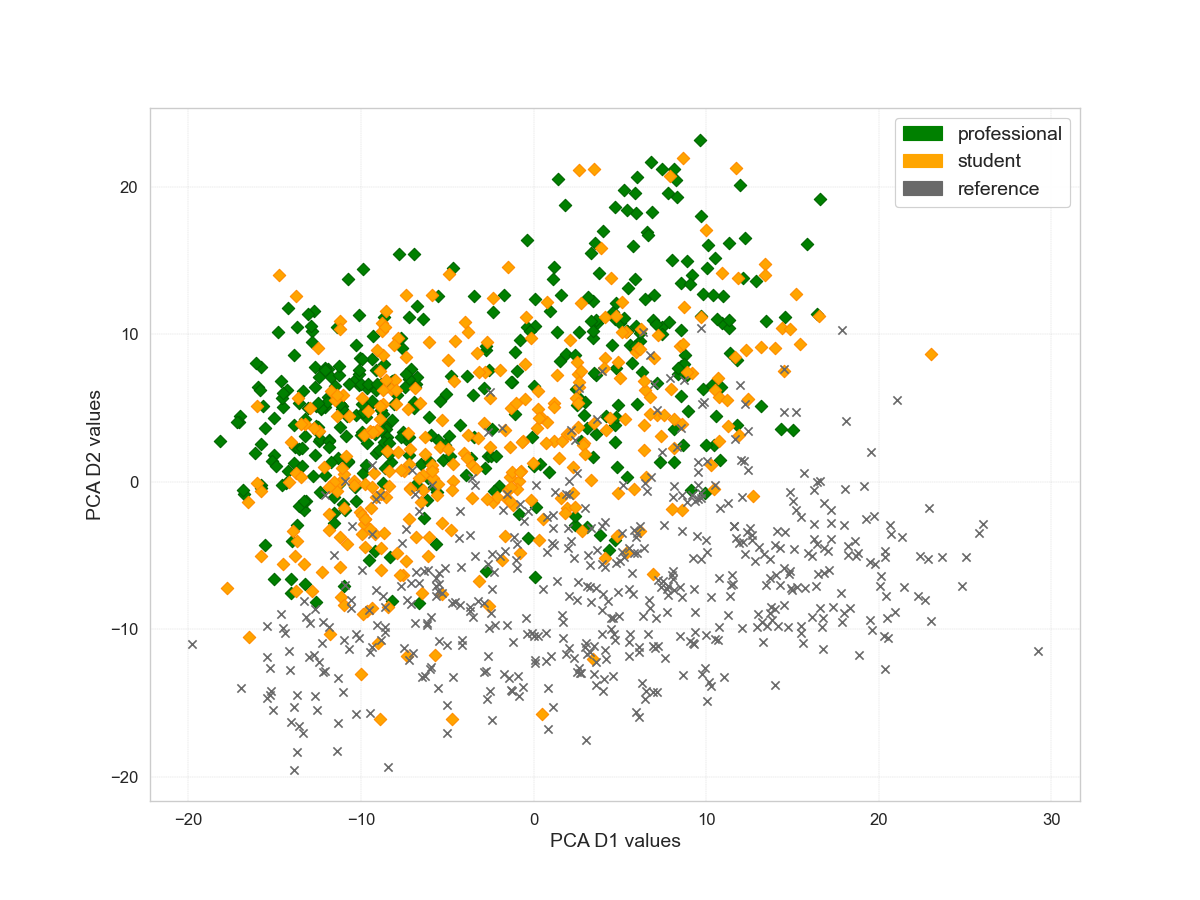
\includegraphics[width=\linewidth]{figures/pca/var-ttype-ruRoberta-large-PCA-scatter}
\end{minipage}
\caption{\label{fig:other}More informative aspects of PCA analysis on other contextualised embeddings}	
\end{figure}

% truth to be told, total variance captured by any dimentions in these representation in ridiculously small: 
%mXLM-R Variance explained per dimension:  [0.07467213 0.06423427]
%TQmono-m Variance explained per dimension:  [0.44481555 0.13820085]
%ruRoberta Variance explained per dimension:  [0.09490415 0.0667047 ] naturally no src

Despite contextualised embeddings seem to capture different aspects of documents relatedness, they achieved the same classification result: there were no significant differences between \textit{TQmono-m, ruRoberta and mdeberta3}, with \textit{stsb-xlm-r-m} being inferior only to \textit{ruRoberta} and \textit{mdeberta3} on professional translations by either SVM or neural classifier. 
On (more challenging) student translations mean-pooled word embeddings (\textit{ruRoberta} and \textit{mdeberta3}) significantly outperformed both sentence embedding models (\textit{TQmono-m} and \textit{stsb-xlm-r-m}) at least by SVM.
% By neural classifier TQmono-m is not different from word-embeddings, while stsb-xlm-r-m significantly loses to all of them

The next section describes UD features from the point of view of their usefulness for translation detection. We report the results of feature selection, based on SVM feature weights and carry out univariate comparisons between text categories to reveal most important translationese indicators and trends that they contribute to. We are going to rely on this analysis in describing the results of professionalism- and quality-related classifications with regard to our main hypothesis that translationese indicators can be related to translation quality.

\section{\label{sec:bestof}Feature Analysis}
This section aims to detect strong translationese predictors among the manually engineered features and provide a linguistic description of translationese in English-to-Russian language pair.
The primary method to achieve this goal is feature selection, supported by univariate feature analysis and statistical significance tests.

Eventually, we want to see whether strong translationese indicators are correlated with professionalism and quality labels/scores and could predict them in a ML setup. 

\subsection{\label{ssec:best_ud}Best of UD features}

\paragraph{\label{par:detect_select}Feature selection}
As discussed above, \gls{RFE} was preferred over \gls{ANOVA} for feature selection because many UD features did not meet the ANOVA requirement of normal distribution and equal variances across compared text categories. In contrast, RFE relies on internal SVM feature weights and gradually prunes less useful ones to reduce the feature set to required N. To infer N experimentally instead of using an arbitrary number of selected features, RFE can be run in a cross-validation setup (RFECV). In our experiments, the algorithm iterated N in the range [3 : size of the feature set], performed 5-fold cross-validation on each N and returned N with the highest mean F1-score across all folds.

%RFECV: Shared best UD features for translation detection (28):
%{'addit', 'ppron', 'nnargs', 'compar', 'attrib', 'nsubj', 'sconj', 'pverbals', 'fixed', 'mark', 'determ', 'finites', 'wdlength', 'acl', 'advmod', 'deverbals', 'acl:relcl', 'copula', 'aux:pass', 'obj', 'amod', 'simple', 'pasttense', 'neg', 'ccomp', 'nmod', 'sentlength', 'advcl'}

% 'deverbals' was #33 that was not reflected in the symmetric weights graph
These experiments returned $N=33$ and $N=42$ for translationese classifications on professional and student translations, respectively. 
After discarding noisy and collinear features, the performance of both classification improved. It went up by 1.3 percentage points from 90.22 to 92.04\% for professional translations, and by 2.1 percentage points from 88.96 to 91.06\% for student translations (based on macro F1 scores). % the statistical differences were not significant in either case on the results of 10 runs in cross-validation setup (on either ttest and on WMW U test, yes, we tried both just in case).

To have a closer look at the commonalities between translation varieties and feature importance in these selections, the lists were intersected and ranked based on the weights assigned by the linear kernel SVM algorithm. Feature weights were obtained from classifiers run on full datasets (without reserving a fraction for testing). Experiments showed that the feature weights were approximately the same if the weights were averaged across the models learnt on each of the folds in a cross-validation setup.

\vspace{-2em}
\begin{figure}[H]
	\centering
	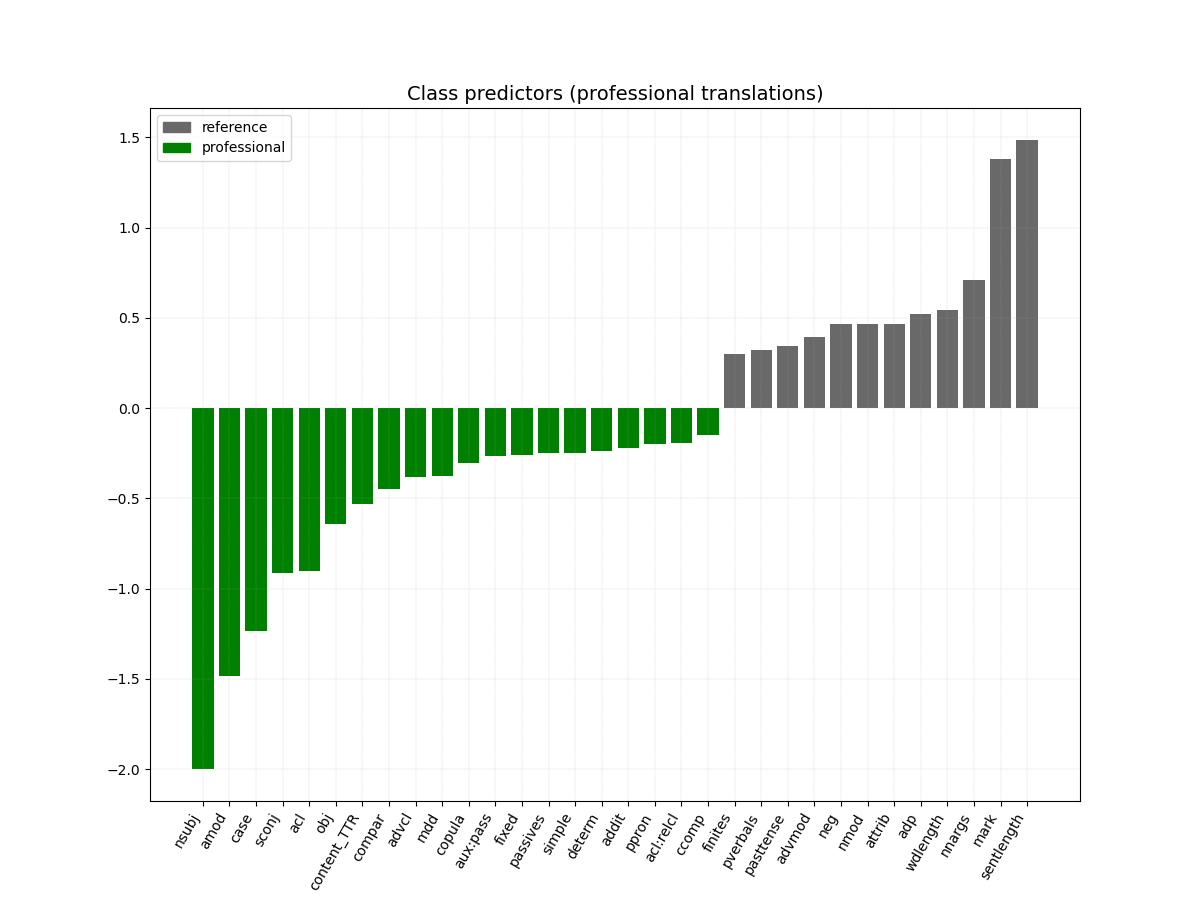
\includegraphics[width=.85\linewidth]{figures/pro-ref-bars-ud33}
	\caption{\label{fig:pro-weights}Weights loading the decision towards each category for 32 RFECV-selected items}	
\end{figure}

Figures~\ref{fig:pro-weights} and~\ref{fig:stu-weights} visualise the weights assigned to the respective subsets of best features in each classification. Features with larger weights can be considered more predictive of the distinctions between categories. 

Detailed explanations of shorthand used on the x-axis can be found in Appendix~\ref{appx:ud}.

\vspace{-2em}
\begin{figure}[H]
	\centering
	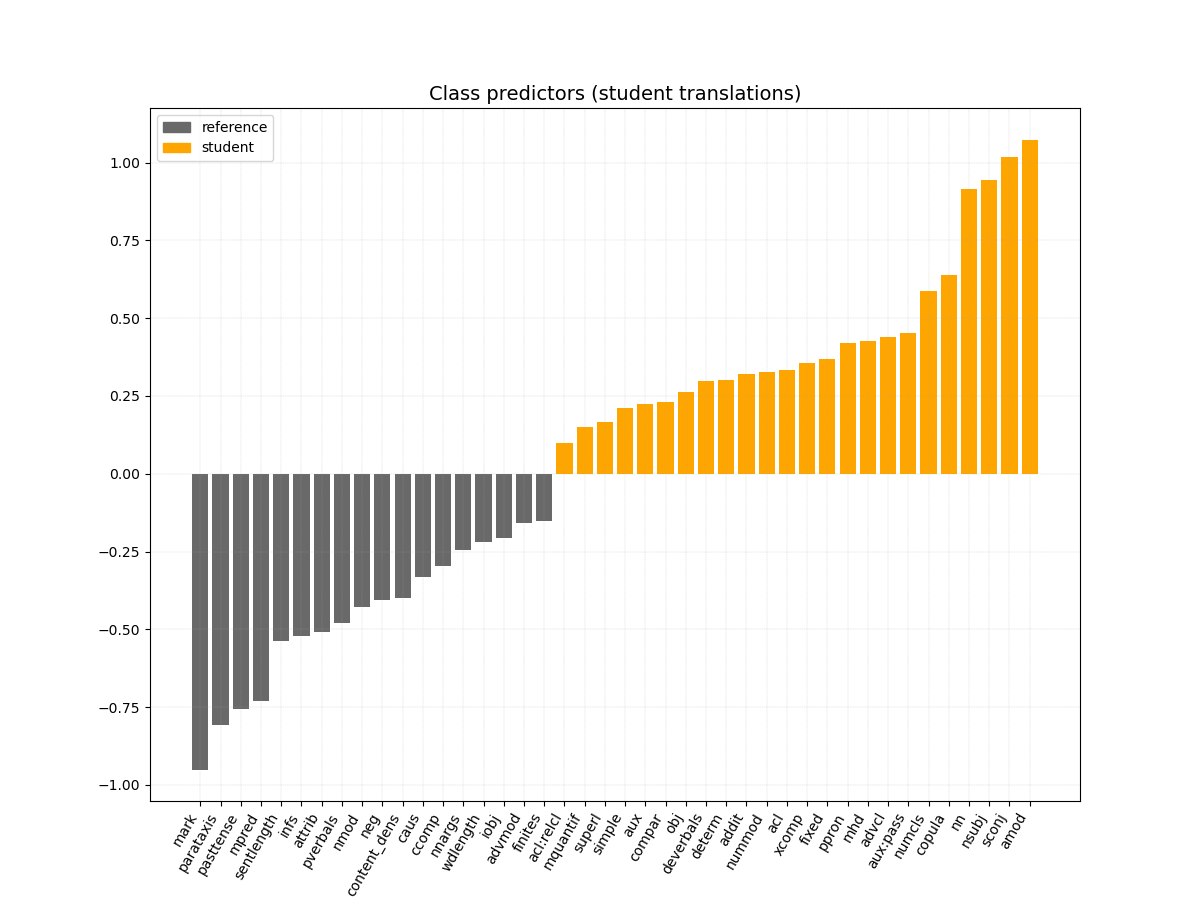
\includegraphics[width=.85\linewidth]{figures/stu-ref-bars-ud42}
	\caption{\label{fig:stu-weights}Weights loading the decision towards each category for 42 RFECV-selected items}	
\end{figure}

%RFECV: Shared best UD features for translation detection (28, sorted by average absolute weight): nsubj, amod, mark, sentlength, sconj, acl, pasttense, attrib, nnargs, copula, obj, nmod, neg, advcl, pverbals, wdlength, aux:pass, compar, fixed, ppron, advmod, addit, determ, deverbals, simple, finites, ccomp, acl:relcl

There were 28 UD features shared between the optimal sets of 33 and 42 translationese indicators in professional and student translationese classifications, respectively. They can be considered strong predictors that capture translational specificity regardless the level of expertise.

The full list of features includes: \textit{amod, sconj, mark, nsubj, pasttense, copula, sentlength, attrib, pverbals, aux:pass, advcl, nmod, ppron, neg, fixed, acl, addit, determ, deverbals, ccomp, obj, nnargs, compar, wdlength, simple, advmod, finites, acl:relcl}.\wlvfootnote{Because the weights for a feature could be quite diverging in professional and student classifications (Spearman correlation was 0.47), the features appear on this list in the descending order according to the absolute weights in the student classification, a hypothetical marked quality class in this research.} 
These features are shown as either `translation predictors' (coloured bars in Figures~\ref{fig:pro-weights} and~\ref{fig:stu-weights}) or `non-translation predictors' (grey bars). Although the weights are shown as loading feature values towards a specific category (reference or translations), it is not clear how this choice is made by the algorithm and this aspect is ignored in our analysis. 
%We were not able to detect any patterns in the data that would explain why some features were weighted to predict translations and others -- non-translations. 

For consideration of space, below we present these 28 features in typological groups, where possible.       

Two-thirds of the features listed above reflected various aspects of sentence structure, rather than frequencies of morphological units. Translationese-related syntactic phenomena were: 
% syntax: amod, mark, nsubj, copula, sentlength, attrib, pverbals, deverbals, advcl, finites, nmod, neg, acl, addit,  ccomp, obj, simple, advmod,  acl:relcl
\begin{description}\compresslist{}
	\item[nsubj, obj:] distribution of core verbal arguments (nominal subjects and objects),
	\item[mark:] frequency of function words that identify another word as a head of a subordinate clause,
	\item[acl:relcl, advcl, acl, ccomp:] frequencies of relative and adverbial clauses, finite and non-finite clauses that modify a nominal or function as clausal complements,  % the issues as he sees them, years to come
	\item[finites, pverbals:] closely related to the previous features, the distributions of finite and non-finite verbal forms in adverbial function, including Russian-specific verb form referred to as a converb (\textcyrillic{\textit{деепричастие}}), a type of participle in the adverbial function,
	\item[deverbals:] ratio of de-verbal nouns, naming of processes, actions, states, to the number of verbs,
	\item[amod, attrib, nmod:] modifiers of noun, including adjectives, participles and other nouns in attributive function (e.g. genitive complement: \textcyrillic{\textit{времена (финансовой) стабильности}} [times of (financial) stability], \textcyrillic{\textit{список грехов}} [list of sins]),
	\item[advmod:] non-clausal adverbial modifier (e.g. \textcyrillic{\textit{но и для выражения сочувствия}} [but also for offering condolences], \textcyrillic{\textit{N существует в виде статичных изображений}} [N exists in static images]),
	\item[simple:] proportion of simple sentences to all sentences in a document, 
	\item[sentlength:] average number of words in a sentence, care was taken to exclude pseudo-sentences that had only numbers and punctuation marks, or contained less than two tokens,
	\item[copula:] function words linking subject to a non-verbal predicate, 
	\item[neg:] negative particles or main sentence negation,
	\item[addit:] additive conjunctions of parenthetical type (such as \textit{what's more, in other words, furthermore, in this regard}), which are optional elements, external to the sentence structure.
\end{description}
Morphological classes, categories and forms, whose quantitative parameters were useful for translation detection, included: 
% morph: sconj, pasttense, aux:pass, ppron, fixed, determ, nnargs, compar, wdlength, 
\begin{description}\compresslist{}
	\item[nnargs:] ratio of nouns or proper names as verb arguments to total of respective functions,
	\item[ppron:] personal pronouns, excluding possessive pronouns,
	\item[sconj:] subordinative conjunctions,
	\item[aux:pass:] analytical passive verb forms
	\item[pasttense:] verbs in past tense,
	\item[fixed:] fixed \gls{MWE}, mostly functional words (e.g. \textcyrillic{\textit{то есть}} [that is]; \textcyrillic{\textit{до сих пор}} [until now]),
	\item[determ:] pronominal determiners (e.g. \textcyrillic{\textit{кaждый}} [every], \textcyrillic{\textit{этот}} [this]),
	\item[compar:] comparative degree of comparison for adjectives and adverbs,
	\item[wdlength:] average number of characters in content words only to avoid co-linearity with features counting various function words.
\end{description}

There were five features that were specific for professional (but not student) translation classification: \textit{adp, passives, mdd, case, content\_TTR}. 
%	\item[case:] function of any syntactic word functioning as case marker (e.g. \textcyrillic{\textit{для полиции; за меньшие деньги}} [for police, for less money]).

To achieve the best result in predicting student translations, SVM considered distributions of 14 more features that were not selected in the classification based on professional translations: \textit{numcls, parataxis, mpred, xcomp, aux, content\_dens, superl, nummod, mhd, iobj, nn, mquantif, infs, caus}. 

Features that were not selected by RFECV for either professional-vs-non-translation or student-vs-non-translations classifications included 13 items. They can be considered less useful for translation detection either due to the lack of considerable distinctions between the categories or due to the collinearity with other features. This list had values for the following features:
%Not selected by RFECV for either pro-ref or stu-ref (13): obl, appos, advers, cconj, discourse, epist, possp, tempseq, flat, anysome, compound, interrog, conj
\begin{description}\compresslist{}\label{pg:rfe_useless}
	\item[tempseq:] cumulative frequency of temporal and sequential connectives (e.g. \textcyrillic{\textit{короче говоря}} [to put it briefly], \textcyrillic{\textit{в конце концов}} [finally, in the end]),
	\item[discourse:] a dependency relation for interjections and other discourse particles (e.g. \textcyrillic{\textit{в первую очередь}} [in the first place], \textcyrillic{\textit{в частности}} [in particular]),
	\item[epist:] epistemic markers of author's stance (e.g. \textcyrillic{\textit{навряд ли}} [unlikely], \textcyrillic{\textit{можно не сомневаться}} [no doubt], \textcyrillic{\textit{вероятно, наверняка}} [probably, definitely]),
	\item[possp:] possessive pronouns,
	\item[cconj, conj:] frequencies of coordinating conjunctions and respective syntactic relation between two conjuncts, 
	\item[advers:] adversative (contrastive) discourse markers (e.g. \textcyrillic{\textit{впрочем}} [however], \textcyrillic{\textit{несмотря на, тем не менее}} [despite, nevertheless])
	\item lexical density, counted as ratio of PoS disambiguated content word types to all tokens,
	\item simple sentences,
	% (e.g. \textcyrillic{\textit{}} [])
	\item[flat, compound:] two types of \gls{MWE}: exocentric semi-fixed sequences such as proper names and dates (e.g. \textcyrillic{\textit{Синдзо Абэ; 24 декабря}} [Shinzo Abe, 24 December]) and endocentric compound MWE, usually hyphenated in Russian (e.g. \textcyrillic{\textit{черно-белый}} [black and white]),
	\item[amod:] non-clausal adjectives and participles functioning as attributes (e.g. \textcyrillic{\textit{финансовый центр}} [financial centre]), % mostly adjectives and participles functioning as attributes, but also "nothing wrong with it", e.g. , удобный гаджет
	\item[obl:] frequency of non-core verbal arguments expressed by a noun (e.g. indirect objects),
	\item[appos:] punctuated or parenthetical modifiers of noun (e.g. \textcyrillic{\textit{мы, демократы}} [we, the democrats], \textcyrillic{\textit{мисс Пигги, персонаж Маппет-шоу}} [miss Piggy, a Mappet show character]),
	\item[interrog:] proportion of sentences ending in question mark,
	\item[anysome:] indefinite and total pronouns (e.g. \textcyrillic{\textit{кому-нибудь, чем-то, когда-то}} [anyone, something, at some point]),

\end{description}

All features on the list above had very weak association with the labels in the range of 0.46 to 0.36, with the exception of oblique nominal objects (\textit{obl}), a non-core verbal argument introduced in Russian by a preposition and, therefore collinear with the frequency of prepositions. Some features on this list seem to disprove a common anticipation by the translation textbooks of deviant use of respective items in translation. However, their use in `translationese' contexts might have been subsumed by other more natural contexts.

%For example, the use of any types of pronouns, especially possessive and indefinite/total is expected to be different under the pressure of the ST. Although our analysis failed to find empiric proof for that, we will be weary of dismissing pronouns as a translationese give-away. It is likely that this feature requires taking into account some context which was ignored in our approach.      

The next paragraph explores the distributional properties of the best translationese indicators revealed in the feature selection process across document categories (translations, sources and non-translations). This contrastive-comparative univariate analysis helps to group features according to specific trends in translational behaviour reflected by the document properties. 

\paragraph{\label{par:featsunivar}Univariate analyses}
To understand more about the prominent patterns of language use in translations picked up by SVM classifiers, we performed a series of statistical tests on individual features identified as strong translationese indicators in the previous paragraph. It is aimed at revealing the impact of the language pair on the linguistic properties of translations. It is known that the distance between the languages is not the only factor that affects translational behaviour, but we do not have the necessary setup to measure the possible contribution from those factors. 
 
For each feature, we compared its distributions in sources, targets and non-translations. The differences were tested for statistical significance using \textit{Mann-Whitney U test for independent samples} and \textit{Wilcoxon signed-rank test} for paired samples of source and target texts. 

First, we identified the features that had significant differences between translations and non-translations (\textit{tgt} and \textit{ref} categories): these are translationese indicators by definition. 
Then, we established whether there were statistically significant differences between the two languages (\textit{src} and \textit{ref} categories) with respect to a given feature, and which language had greater values.
Finally, for each feature, we performed pairwise comparisons between frequencies in translations and in each of the languages.

The outcome of the above sequence of tests can be viewed as capturing the amount of effort invested by a translator to reconcile differences between the two languages (if any) for a given feature. The features, representing various trends in translational behaviour, can be arranged in three major groups (see Table~\ref{tab:trends}), depending on the adopted translation strategy and the scale of its implementation. 

\begin{longtable}[H]{l|l|p{3cm}p{8cm}}
%		\begin{tabular}
			\toprule		
		& group & trend & description \\
			\midrule
	\parbox[t]{2mm}{\multirow{20}{*}{\rotatebox[origin=c]{90}{high ------------ amount of effort ------------ low}}}	&	\multirow{3}{*}{reproducing ST}& anglicisation (ref<src<tgt)& TT values greater than in SL and much greater than in TL, possibly the use of SL patterns even when unprompted \\
	\cmidrule{3-4}
	% ref<src=tgt
		&	& shining-through ref<tgt=src & No difference between ST and TT values, both are higher than in TL \\
		\cmidrule{3-4}
		&	& overuse of SL ref<tgt<src & Many translation decisions are prompted by ST, which has higher values than in TL \\
		\cmidrule{2-4}
		&	\multirow{4}{*}{counteracting ST} &  underuse of TL tgt<=src<ref & Lack of effort to add typical TL items when not prompted by ST \\
		\cmidrule{3-4}
		&	& normalisation src<=tgt<ref & Insufficient efforts to bring ST frequencies in line with TL norm \\
		\cmidrule{3-4}
		&	& russification src<ref<tgt tgt<ref<src & Active use of TL patterns unseen in ST or effective counteraction of ST influence leading to overuse of TL items \\
		\cmidrule{3-4}
		&	& adaptation tgt=ref<src src<ref=tgt & No translationese: significant differences between the two languages are reconciled in favour of the TL norm \\
		\cmidrule{2-4}
		& third code & SL/TL-independent tgt<ref=src ref=src<tgt & Translationese features with significant differences from both languages and no language gap \\
			\bottomrule
%		\end{tabular}
		\caption{\label{tab:trends}Patterns in translational behaviour}\\
\end{longtable}

Besides, there was a group of features that were useless for a translationese study, because they had the same frequencies in translations and non-translations, and also did not distinguish the languages. In the classification based on professional translations this group included frequencies of adpositions (prepositions) and discourse particles such as interjections. In student translation data there were no statistically significant differences between document categories for interrogative sentences and adverbial quantifiers (e.g. \textcyrillic{\textit{совершенно}} [entirely],  \textcyrillic{\textit{чрезмерно}} [utterly]).

Further on, we established the strength of association between each feature values and binary categorical labels (translation, non-translation) by measuring the quality of single-feature Logistic Regression classifier using macro F1-score (LogR). The results of significance tests and variable-label association analysis are collected in Table~\ref{tab:shared_rfecv_feats}. The features selected by RFECV are sorted by LogR F1-score averaged for students and professionals. Statistically significant results are indicated by \textit{less-than} and \textit{greater-than} signs, the lack thereof is shown with an \textit{equals} sign.

With regard to the strength of association between feature values and class labels (translations, non-translations), only half of shared features from RFECV selections yield F1-scores above the chance level (0.5) when used in a single-feature classifier (shown in bold in Table~\ref{tab:shared_rfecv_feats}).
%in a similar recent study \cite{Hu2021} reached an accuracy of 96.55\% on 160 cohesive markers alone
%how discriminative these characteristics are?
% does a feature typify O or T according to a log-likelihood (LL)? I need raw counts for that, I have only normalised frequencies, some values are not freqs at all!
\begin{longtable}[H]{p{1.6cm}|ccc||ccc}
	\toprule
		      &      \multicolumn{3}{c}{Professional} 	&      \multicolumn{3}{c}{Student}\\
	\midrule
	feature & LogR & trend & means   & LogR & trend   & means   \\
	\midrule
	\textbf{nsubj}   & \textbf{0.82} & overuse of SL  & ref\textless{}tgt\textless{}src & \textbf{0.71} & shining & ref\textless{}tgt=src  \\
	\textbf{mark} & \textbf{0.74} & overuse of SL  & ref\textless{}tgt\textless{}src & \textbf{0.68} & overuse of SL & ref\textless{}tgt\textless{}src \\
	\textbf{acl:relcl}  & \textbf{0.69} & overuse of SL  & ref\textless{}tgt\textless{}src & \textbf{0.66} & overuse of SL & ref\textless{}tgt\textless{}src \\
	\textbf{advcl}   & \textbf{0.7}  & overuse of SL  & ref\textless{}tgt\textless{}src & \textbf{0.63} & overuse of SL & ref\textless{}tgt\textless{}src \\
	\textbf{obj}  & \textbf{0.72} & overuse of SL  & ref\textless{}tgt\textless{}src & \textbf{0.61} & overuse of SL & ref\textless{}tgt\textless{}src \\
	\textbf{fixed}   & \textbf{0.56} & russification  & src\textless{}ref\textless{}tgt & \textbf{0.58} & russification & src\textless{}ref\textless{}tgt \\
	sentlength & \textbf{0.61} & NA  & ref\textless{}tgt & \textbf{0.57} & NA & ref\textless{}tgt \\
	\textbf{acl}  & \textbf{0.62} & shining  & ref\textless{}src=tgt  & \textbf{0.56} & shining & ref\textless{}src=tgt  \\
	\textbf{nnargs}  & \textbf{0.68} & normalisation  & src\textless{}tgt\textless{}ref & \textbf{0.55} & normalisation & src\textless{}tgt\textless{}ref \\
	\textbf{amod} & \textbf{0.51} & russification  & src\textless{}ref\textless{}tgt & \textbf{0.53} & russification & src\textless{}ref\textless{}tgt \\
	\textbf{attrib}  & \textbf{0.51} & russification  & src\textless{}ref\textless{}tgt & \textbf{0.52} & russification & src\textless{}ref\textless{}tgt \\
	\textbf{copula}  & \textbf{0.52} & overuse of SL  & ref\textless{}tgt\textless{}src & \textbf{0.51} & overuse of SL & ref\textless{}tgt\textless{}src \\
	\textbf{ccomp}   & \textbf{0.63} & overuse of SL  & ref\textless{}tgt\textless{}src & \textbf{0.5}  & overuse of SL & ref\textless{}tgt\textless{}src \\
	\textbf{nmod} & 0.36 & adaptation  & src\textless{}ref=tgt  & \textbf{0.5}  & russification & src\textless{}ref\textless{}tgt \\
	deverbals  & 0.45 & normalisation  & src\textless{}tgt\textless{}ref & 0.45 & russification & src\textless{}ref\textless{}tgt \\
	addit   & 0.4  & shining  & ref\textless{}src=tgt  & 0.43 & SL/TL-indep   & ref=src\textless{}tgt  \\
	wdlength   & 0.4  & NA  & tgt\textless{}ref & 0.43 & NA & ref\textless{}tgt \\
	pasttense  & \textbf{0.51} & SL/TL-indep & tgt\textless{}ref=src  & 0.42 & SL/TL-indep   & tgt\textless{}ref=src  \\
	neg  & 0.41 & normalisation  & src\textless{}tgt\textless{}ref & 0.4  & normalisation & src\textless{}tgt\textless{}ref \\
	advmod  & \textbf{0.53} & overuse of SL  & ref\textless{}tgt\textless{}src & 0.38 & SL/TL-indep   & tgt\textless{}ref=src  \\
	aux:pass   & 0.36 & russification  & tgt\textless{}ref\textless{}src & 0.38 & adaptation & tgt=ref\textless{}src  \\
	compar  & 0.38 & overuse of SL  & ref\textless{}tgt\textless{}src & 0.38 & overuse of SL & ref\textless{}tgt\textless{}src \\
	finites & 0.36 & adaptation  & tgt=ref\textless{}src  & 0.38 & overuse of SL & ref\textless{}tgt\textless{}src \\
	determ  & 0.36 & overuse of SL  & ref\textless{}tgt\textless{}src & 0.37 & overuse of SL & ref\textless{}tgt\textless{}src \\
	ppron   & 0.36 & overuse of SL  & ref\textless{}tgt\textless{}src & 0.37 & overuse of SL & ref\textless{}tgt\textless{}src \\
	pverbals   & 0.36 & adaptation  & src\textless{}ref=tgt  & 0.37 & adaptation & src\textless{}ref=tgt  \\
	sconj   & 0.36 & russification  & src\textless{}ref\textless{}tgt & 0.37 & russification & src\textless{}ref\textless{}tgt \\
	simple  & \textbf{0.67} & underuse of TL & tgt\textless{}src\textless{}ref & 0.37 & underuse of TL & tgt\textless{}ref\textless{}src \\
	\bottomrule
	\caption{\label{tab:shared_rfecv_feats}Properties of 28 UD features identified as discriminative between translations and non-translations by RFECV}\\
\end{longtable}

Table~\ref{tab:shared_rfecv_feats} shows that the more salient deviations from non-translation for both translation varieties can be described by the same trends. 

Half of translationese indicators in both translation collections had frequencies, which were shifted towards SL value and were higher than expected in the TL. In these cases translators seem to reproduce patterns observed in the SL (overuse of SL patterns, shining-through or anglicisation). 
For example, the overuse of SL patterns was seen for \textit{nsubj, mark, acl:relcl, advcl, obj}.  

A different translational trend is associated with features, where translators actively counteract the influence of the ST and bring the frequencies in translations closer to the TL norm. Underuse of TL items, normalisation, russification and adaptation together explain 13 (professionals) and 12 (students) out of 28 translationese indicators. 

A few features (\textit{pasttense} and \textit{advmod, addit} in student translations) can be described as contributing to \textbf{SL/TL-independent translationese}. This group represents the trends in translational behaviour that can be explained by factors other than SL/TL contrast. 

For some features, sources and TL reference compare differently in professional and student translations. It may or may not result in changes in their interpretation in terms of investigated translational trends. 
For example, both professionals and students generated fewer simple sentences than can be expected in the TL. However, professional translators faced a much more challenging situation: their sources had fewer simple sentences than in the TL to start with. Students, on the contrary, did not have to overcome the pressure of the ST as their sources had more simple sentences than in the TL. Nonetheless, students demonstrated a known translational behaviour to use longer sentences with multiple clauses and converted the surplus of simple sentences into the lack of thereof with regard to the TL norm. 
% pro simple : src 0.29 +/-0.10  tgt 0.23 +/-0.09  ref 0.31 +/-0.10
% stu simple : src 0.34 +/-0.14  tgt 0.29 +/-0.13  ref 0.31 +/-0.10

The case of additive discourse markers (\textit{addit}) is another example of how ST properties can impact the outcomes of this analysis. Professionals seem to have carried over the additive markers that were seen in the source texts, while students' behaviour was indeed divergent from both ST and TL: students generated surplus additive markers where they were not seen in sources. Overuse of overt linking parentheticals is a known problem of novice writers and translators, who rely on `crude force', using external markers of cohesion instead of making efforts towards a better sentence structure.  
%pro addit: ref<src=tgt src 0.09 +/-0.06 tgt 0.09 +/-0.07 ref 0.08 +/-0.06
%stu addit: ref=src<tgt src 0.08 +/-0.09 tgt 0.10 +/-0.09 ref 0.08 +/-0.06

An anticipated outcome of the analysis is seen for analytical passives (\textit{aux:pass}). Both students and professionals avoid carrying over English passive form, which has a corresponding form in Russian. However, professionals view the legitimate isomorphic Russian form as less acceptable, which leads to the lack of it in translations (as compared to non-translations). Both professionals and students seem to make efforts to replace English analytical passives with either of the other three Russian means to express passive relations as can be seen from the frequencies for overall counts for passive forms (see \textit{passives} in Table~\ref{tab:spec_rfecv_feats}). Interestingly, textbooks on practical translations from English into Russian tend to emphasise passives as a typical source of less fluent translation solutions. Some authors make it appear that there are more passive constructions in English than in Russian~\cite[see, for example,][]{Zrazhevskaya1972, Belyaev2010, Borisova2019}. We have seen, however, that it is only true for analytical passives.
% I have a lot of examples for analytical passives avoided in professional translations in "not analytical passives in prof translations" note in Nixnote.

The strength of association for most features is higher for professional than for student translations. We attribute this to structural simplicity of the source texts, offered to students, on the one hand, and to the difference in the size of the underlying subcorpora, on the other. As demonstrated in Table~\ref{tab:corpus_means}, student translations had fewer instances, the smallest mean document length in tokens and in number of sentences, and at the same time the largest STD for both parameters. Smaller corpus size could have contributed to the sparsity of investigated features.

\begin{table}[H]
	\begin{tabular}{l|llll}
			\toprule
			subcorpus                 & docs & tokens per doc   & tokens per sent & sent per doc  \\
			\midrule
			student translations      & 334  & 646.88 +/-984.07  & 22.39 +/-4.81    & 29.68 +/-40.68 \\
			professional translations & 404  & 950.45 +/-282.42  & 22.95 +/-4.03    & 42.44 +/-13.42 \\
			non-translations          & 497  & 1053.80 +/-539.18 & 20.48 +/-3.04    & 52.39 +/-26.73 \\
			\bottomrule
		\end{tabular}
 \caption{\label{tab:corpus_means}Additional corpus parameters for translationese classifications}
\end{table}

Besides, student translations were more diverse in the types of translation solutions attempted for typical translation problems. Their renditions were less predictable than stable choices by professional translators, which resulted in a greater spread of values on translationese indicators. 

%However, a few features managed to overcome the disadvantages of shorter documents and lower homogeneity of student translation collection and demonstrated stronger association with the class labels for student than for professional translations (e.g. \textit{fixed, amod, attrib, nmod, addit}). We hypothesise that they capture strong quality-related signals. \todo[inline]{Double check this!}  

%We decided against artificially reducing the length of document-size outliers in student collection because it would mean interfering with the intersecting quality-annotated subsets. 

To complete the overview of UD features usefulness for translationese classification, we offer a description of translationese indicators that were specific for detecting either professional or student translations.  

Table~\ref{tab:spec_rfecv_feats} gives contrastive-comparative profiles for the features that were specific for each translation collection in the translationese classification. The table is sorted by F1-score in the respective classification. Equals sign in \textit{means} column indicates no statistical differences between the shorthanded categories. Again, features that were selected as best predictors of student translations against non-translations and had above-chance association with the label are shown in bold.

%Specific to PRO-REF (5): case, mdd, passives, content_TTR, adp

%Specific to STU-REF (14): numcls, parataxis, mpred, xcomp, aux, content_dens, superl, nummod, mhd, iobj, nn, mquantif, infs, caus

\begin{longtable}[H]{p{1.84cm}|ccc||ccc}
	\toprule
	&      \multicolumn{3}{c}{Professional} 	&      \multicolumn{3}{c}{Student}\\
	\midrule
	feature & LogR & group & means   & LogR & group   & means   \\
	\midrule
	\multicolumn{7}{c}{Features specific for professional vs non-translation classification} \\
	\midrule
	mdd           & \textbf{0.57} & overuse of SL & ref\textless{}tgt\textless{}src & 0.39 & overuse of SL  & ref\textless{}tgt\textless{}src \\
	case          & \textbf{0.54} & overuse of SL & ref\textless{}tgt\textless{}src & \textbf{0.54} & overuse of SL  & ref\textless{}tgt\textless{}src \\
	adp           & 0.36 & \textbf{useless}       & tgt=ref=src                     & 0.37 & adaptation     & tgt=ref\textless{}src           \\
	cont-TTR  & 0.36 & adaptation    & src\textless{}ref=tgt           & 0.37 & underuse of TL & tgt\textless{}src\textless{}ref \\
	passives      & 0.36 & normalisation & src\textless{}tgt\textless{}ref & 0.37 & normalisation  & src\textless{}tgt\textless{}ref \\
	\midrule
	\multicolumn{7}{c}{Features specific for student vs non-translation classification} \\
	\midrule
	\textbf{parataxis}     & 0.37 & adaptation    & src\textless{}ref=tgt           & \textbf{0.67} & normalisation & src\textless{}tgt\textless{}ref \\
	\textbf{mhd}           & \textbf{0.63} & SL/TL-indep   & ref=src\textless{}tgt           & \textbf{0.63} & SL/TL-indep   & ref=src\textless{}tgt           \\
	\textbf{numcls}        & \textbf{0.71} & anglicisation & ref\textless{}src\textless{}tgt & \textbf{0.52} & russification & src\textless{}ref\textless{}tgt \\
	\textbf{xcomp}         & \textbf{0.68} & shining       & ref\textless{}src=tgt           & \textbf{0.52} & shining       & ref\textless{}src=tgt           \\
	mpred         & \textbf{0.53} & overuse of SL & ref\textless{}tgt\textless{}src & 0.44 & overuse of SL & ref\textless{}tgt\textless{}src \\
	aux           & 0.42 & overuse of SL & ref\textless{}tgt\textless{}src & 0.4  & adaptation    & tgt=ref\textless{}src           \\
	nummod        & 0.46 & shining       & src=tgt\textless{}ref           & 0.38 & adaptation    & src\textless{}ref=tgt           \\
	iobj          & \textbf{0.58} & russification & src\textless{}ref\textless{}tgt & 0.37 & normalisation & src\textless{}tgt\textless{}ref \\
	infs          & 0.39 & russification & src\textless{}ref\textless{}tgt & 0.37 & adaptation    & src\textless{}ref=tgt           \\
	nn            & 0.38 & normalisation & src\textless{}tgt\textless{}ref & 0.37 & russification & src\textless{}ref\textless{}tgt \\
	caus          & 0.36 & russification & src\textless{}ref\textless{}tgt & 0.37 & normalisation & src\textless{}tgt\textless{}ref \\
	cont-dens & 0.36 & normalisation & src\textless{}tgt\textless{}ref & 0.37 & russification & src\textless{}ref\textless{}tgt \\
	mquantif      & 0.36 & shining       & ref\textless{}src=tgt           & 0.37 & \textbf{useless}       & tgt=ref=src                     \\
	superl        & 0.36 & adaptation    & tgt=ref\textless{}src           & 0.37 & adaptation    & tgt=ref\textless{}src  \\
	\bottomrule
	\caption{\label{tab:spec_rfecv_feats}Properties of five and 14 UD features that were unique for professional and student experiments}\\
\end{longtable}	

Quite surprisingly, RFECV selections of features specific for either professional or student translation classification included features that were useless in that particular setting from the point of view of univariate analysis (see \hyperlink{ft:adp}{adp} and \hyperlink{ft:mquantif}{mquantif}). This might mean that they were employed as part of a multivariate pattern detected by an algorithm.

Some features were not selected for a particular classification despite being well-associated with the class. For example, number of clauses (\textit{numcls}), mean hierarchical distance (\textit{mhd}) and frequency of clausal complements without subjects (\textit{xcomp}) had F1-score over 0.63 when used in a single-feature classifier for professional translations vs reference, but were not selected by RFECV algorithm in that classification. Most likely these features, ignored by RFECV, were collinear with other features in the data. Number of clauses is negatively correlated with ratio of simple sentences. 

\textit{Xcomp} was well-correlated with infinitives and number of modal predicates, because it mostly captured typical cases of transferring English modal verbs into Russian, where in non-translations other ways of expressing subjective modality would be used. Example~\ref{ex:mpred} has a case of positive transfer of a modal predicate, where a more fluent rendition could be \textcyrillic{Ошибки нельзя исправить.} [It is impossible to correct errors]. 

\ex. \label{ex:mpred}\hspace{1pt}
[about death penalty] Mistakes can never be rectified.\\
\textcyrillic{Ошибки не могут быть исправлены.}\\
`Mistakes cannot be corrected'.

This typical example also demonstrates the multivariate nature of translationese. Following the English pattern in cases like in Example~\ref{ex:mpred} drives up the counts for analytical passives and \textit{xcomp}.

Among the 13 UD features that were discarded by RFECV as useless in both classifications (see page~\pageref{pg:rfe_useless}), only one feature -- \textit{frequency of non-core verbal argument} (\textit{obl}) -- showed reasonably high correlation with the class (F1-score of 0.64 and 0.59 for professional and student classification, respectively). This can be explained by its collinearity with adpositions because oblique nominal objects are introduced by this class of function words. 


% To test this hypothesis we built a corelation matrix and visualised it as a heatmap in Fugure~\ref{fig:heat_collinear}.

%Not selected by RFECV for either pro-ref or stu-ref (13): obl, appos, advers, cconj, discourse, epist, possp, tempseq, flat, anysome, compound, interrog, conj

%\begin{longtable}[H]{p{1.84cm}|ccc||ccc}
%	\toprule
%	&      \multicolumn{3}{c}{Professional} 	&      \multicolumn{3}{c}{Student}\\
%	\midrule
%	feature & LogR & trend & means   & LogR & trend   & means   \\
%	\midrule
%		feature   & LogR-F1 & trend         & means                           & LogR-F1 & trend          & means                           \\
%		obl       & \textbf{0.64}    & russification & src\textless{}ref\textless{}tgt & \textbf{0.59}    & russification  & src\textless{}ref\textless{}tgt \\
%		epist     & 0.45    & anglicisation & ref\textless{}src\textless{}tgt & 0.37    & adaptation     & tgt=ref\textless{}src           \\
%		advers    & 0.39    & overuse of SL & ref\textless{}tgt\textless{}src & 0.37    & adaptation     & tgt=ref\textless{}src           \\
%		appos     & 0.39    & SL/TL-indep   & tgt\textless{}ref=src           & 0.37    & underuse of TL & tgt=src\textless{}ref           \\
%		interrog  & 0.39    & shining       & ref\textless{}tgt=src           & 0.38    & useless        & tgt=ref=src                     \\
%		conj      & 0.37    & SL/TL-indep   & ref\textless{}tgt=src*          & 0.46    & SL/TL-indep    & ref=src\textless{}tgt           \\
%		anysome   & 0.36    & overuse of SL & ref\textless{}tgt\textless{}src & 0.37    & adaptation     & tgt=ref\textless{}src           \\
%		cconj     & 0.36    & adaptation    & tgt=ref\textless{}src           & 0.37    & adaptation     & tgt=ref\textless{}src           \\
%		compound  & 0.36    & adaptation    & tgt=ref\textless{}src           & 0.37    & russification  & tgt\textless{}ref\textless{}src \\
%		discourse & 0.36    & useless       & tgt=ref=src                     & 0.37    & underuse of TL & tgt=src\textless{}ref           \\
%		flat      & 0.36    & russification & tgt\textless{}ref\textless{}src & 0.37    & russification  & tgt\textless{}ref\textless{}src \\
%		possp     & 0.36    & russification & src\textless{}ref\textless{}tgt & 0.37    & adaptation     & src\textless{}ref=tgt           \\
%		tempseq   & 0.36    & adaptation    & tgt=ref\textless{}src           & 0.37    & adaptation     & tgt=ref\textless{}src  \\
%		\bottomrule
%		\caption{\label{tab:useless_rfecv_feats}Properties of 13 UD features discarded as useless by RFECV in both translationese classifications. Equals sign indicates no statistical differences. * marks cases where ref=src}\\        
%\end{longtable}	

For consistency, we added the results for full alphabetised list of features in separate tables for each translation variety in Appendix~\ref{appx:feat_analysis}.  

Drawing conclusions from analysis of UD features, we will focus on properties of student translations as the more relevant variety for the subsequent TQ tasks. We found that the outcomes of translationese classifiers on student and professional translations were affected by the differences in the underlying source text collections. Students seem to have worked with shorter and structurally less challenging documents that were more similar to the reference corpus. 
We can hypothesise that students also generated a wider range of renditions for typical translation problems which made them more diverse as a category and less predictable.

RFECV revealed 42 strong translationese predictors for student translations. Two thirds of them were also found useful to detect professional translations. Only 17 features out of 42 had a reasonably high association with translation/non-translation class labels. The F1-score in a single-feature LogR classifier was in the range of 0.5 to 0.71. 

Nine of these individually well-associated 17 features represented a tendency to carry over ST properties into the target text (overuse of ST patterns and shining-through)\wlvfootnote{inc. shining-through indicators: \textit{acl:relcl, acl, advcl, ccomp, copula, mark, obj, nsubj, xcomp}}. Seven more features reflected the tendency to avoid isomorphic (structurally parallel) solutions in favour of the options more typical for the TL (normalisation), which sometimes makes translations over-emphasise TL properties (russification)\wlvfootnote{\textit{amod, attrib, fixed, nmod, nnargs, numcls, parataxis}}. One feature (\textit{mean hierarchical distance}) in this set had frequencies dissimilar to both ST and TL.
We excluded sentence length and word length from this analysis because these parameters are imposed by the language system, which undermines their usefulness for the proposed analysis, at least in the part of cross-linguistic comparisons.

Analysis of translationese trends should be taken with a grain of salt. Our setup did not allow to test for other possible constraints that affect decision-making in translation apart from SL-TL contrast (e.g. cognitive load, language prestige and established norms). A dramatic decrease in the ratio of simple sentences and changes in the values of the associated properties (most notably, total number of clauses and number of explicit syntactic subjects) is likely to capture a more universal tendency to sentence lengthening and increased syntactic complexity in translations, which is not specific to the given language pair. 
% maybe add colinearity heatmap to for Spearman corr between each pair of features using thir indices from Appx1 as ticks

\subsection{\label{ssec:best_collgram}Best of collgram features} 

Despite comparatively poor performance of \textit{collgram} features, an attempt was made to identify components with higher predictive power. \gls{RFECV} algorithm which determines the optimal number of features (instead of setting N a-priori), could not find any features to exclude to achieve better results for either of the translationese classifications. It means that features included in \textit{collgram} set were equally useful/useless. 

%%% this interpretation is speculative: we decided that we don't understand why features are weighted towards T or O class.
%Reducing this feature set to six best features revealed some commonalities between student and professional translations. In particular, the algorithm selected \textit{average t-score of all detected bigram collocations} and \textit{the t-score-based ratio of all detected bigram collocations to all bigrams} as indicators of translations. A shared predictor of non-translations class was \textit{average NPMI score of all detected bigram collocations}. Although the signal was quite weak, we can tentatively suggest that collocational measures based on t-score  captured the specificity of translational language a bit better.  
%If we recall our reasoning for including collocational features (page~\pageref{pg:why_collocations}), this observation confirms that translations had more prominent patterns of high-frequency words, while non-translations had more stable patterns of lower-frequency words sequences. 


%% 70.33 -> 71.92
%%pro 4 ['av_bigram-tscore>0', '%bigram-tscore>0', '%trigram-tscore_absent', '%bigram-npmi_absent']
%%ref 2 ['av_bigram-npmi>0', '%trigram-tscore>6.0']
%
%% over one percentage point down to 62.34
%%stu 4 ['av_bigram-tscore>0', '%bigram-tscore>0', 'trigram-npmi_std',   '%trigram-npmi_absent']
%%ref 2 ['av_bigram-npmi>0', 'av_trigram-npmi>0']

% pro and stu intersection, when N=6: 'av_bigram-tscore>0', '%bigram-tscore>0', 'av_bigram-npmi>0',
%
The poor performance of collocational features indicates that they are unable to effectively pick theoretically expected collocational differences between translations and originally-authored texts. Indeed, the estimated effect size for (statistically significant) differences between categories on most of these features was small. As explained above, we measured the association between a variable and a category label using F1-score from a single-feature \textit{Logistic regression} classifier. 
In classification on professional translations there were only four features with this score over 0.52 (\textit{bigram-tscore\_std, av\_bigram-tscore>0, av\_trigram-tscore>0, trigram-tscore\_std}), while for student translations only one feature surpassed F1=0.46 (\textit{trigram-tscore\_std}\footnote{standard deviation for the association scores in each document}). 

We noticed that values for these most successful collocational features were lower in translations (professional or student) that in non-translations. In fact, lower values for translations are observed for all statistically significant differences in this feature set, except for OOV ratios. No statistical differences were found for features that capture the ratio of negatively-collocated items. 

These observations seem to indicate that translations tend to have lower ratios of recognisable collocations of any type (i.e. measured by either NPMI or t-score) than non-translations. The collocations found in translations are less stable and less varied in terms of association strength. The strongest translation predictor in this feature set is OOV ratio, i.e. the proportion of collocations not attested in the non-translated TL.

%Which is unexpected -- Nope!. Can it be a function of document length in sentences?? No, I don't see impressive differences in number of sentences per document: ref 20.1, stu 21.8, pro 22.4
%% Average sentence length is also similar and as expected ref 20.46 (3.06), stu 22.39 (4.81), pro 22.95 (4.03)
%
%% pro-ref
%% logreg_f1(tgt,ref) > 0.52 was seen for trigram-tscore_std, av_trigram-tscore>0, av_bigram-tscore>0,  bigram-tscore_std, non-translations values always higher
%
%% stu-ref
%%logreg_f1(tgt,ref) > 0.46 trigram-tscore_std

\subsection{\label{ssec:best_ngram}Best of n-gram features} 
The observations on better-performing features from n-gram feature set, confirmed that, compared to non-translations, translations had significantly higher proportions of bigrams and trigrams not attested in a large TL model (up to 60 and 61\% for trigrams in professional and students vs 56\% in the comparable non-translations subset). The ratios of OOV was a relatively strong predictor of the category as was the case with collocations: there were more unseen bigrams and trigrams in translations than in non-translations. % 26\% and 24\% for bigrams vs 23\% in non-translations. STD for these averages were quite low, not more than 6\%.

We observed that any features based on unigrams performed worse than on bigrams, followed by trigrams. 
Similarly, ratios of bigrams/trigrams from the bottom-frequency quartiles had less predictive power in either of our translation detection setups than from top-frequency quartiles.

Note that the subset of non-translations (ref) used in the classification experiments was not intersecting with the resource used to train TL n-gram model. Besides, recall that we replaced all proper names and their sequences with a PROPN tag to reduce the expected impact of foreign names on these counts.
The values for these features were quite consistent across all documents in each category and had STD of not more than 6\%.

%nbest 6 RFE
%F1-score:
%86.04 (+/-2.99) -> 85.60 (+/-2.90)
%pro 5 ['trioov', 'bifreq', 'trifreq', 'pplex', 'bioov']
%ref 1 ['sdpplex']
%
%F1-score:
%85.61 (+/-3.70) -> 85.12 (+/-4.29)
%ref 1 ['sdpplex']
%stu 5 ['bioov', 'pplex', 'trifreq', 'bifreq', 'trioov']union
\label{pg:stu_more_surprising_than_pro}
Quite unexpectedly, average n-gram LM sentence perplexity (as calculated with \textit{KenLM} library) was higher for non-translations than for translations, and student translations were closer to originally-authored documents (cf. professionals: 3,677.36, students: 4,310.06, non-translations: 5,452.89). It should be noted that sentence perplexity scores varied a lot from sentence to sentence in a document. In non-translations subcorpus, the average STD for a document was the largest and reached 15105.84, three times larger than the mean.
This can indicate a higher lexical variety of original texts and a relatively limited, standardised word choice in professional translations. Student translations, on the one hand, might contain more cases of unexpected lexical strings, including spelling errors. 
This finding is at odds with results reported by~\cite{Bizzoni2021}, who compared student and professional translations from English into German. They were surprised to find that professional translations had higher values for LM perplexity than student translations.

The sets of features most associated with the category revealed by single-feature classifiers had only two features in common for classifications based on student and professional translations (trioov, trifreq), with student translations being more challenging.

Summarising the performance of abstract lexical features, we can report that student and professional translations shared three \textit{collgram} features identified by RFE (with N=6) as having the highest predictive power (\textit{av\_bigram-tscore>0, \%bigram-tscore>0, av\_bigram-npmi>0}). In the n-gram feature set all six selected features were shared (\textit{bioov, pplex, trifreq, bifreq, trioov, sdpplex}). 

In univariate analysis, there were two collgram and two shared n-gram features reasonable well-associated with the category.
% collgram: trigram-tscore_std, av_bigram-tscore>0
% ngram: trioov, trifreq

The union of outcomes of feature selection and univariate analysis gives a list of 10 best translationese indicators out of the total of 34 features in \textit{collgram} and \textit{n-gram} feature sets.
% av_bigram-npmi>0, av_bigram-tscore>0, %bigram-tscore>0, trigram-tscore_std, bifreq, bioov, trifreq, trioov, pplex, sdpplex
\begin{description}\compresslist{}
	\item[1. av\_bigram-npmi>0:] average NMPI score for all positively scored bigrams in the document,
	\item[2. av\_bigram-tscore>0:] average t-score for all positively scored bigrams in the document,
	\item[3. \%bigram-tscore>0:] ratio of all identified bigrams (based on t-score) to the length of the document (in tokens),
	\item[4. trigram-tscore\_std:] standard deviation for the association scores in each document,
	
	\item[5. bifreq:] ratio of bigrams in the top frequency quartile (based on a large non-translated TL corpus),
	\item[6. bioov:] ratio of bigrams absent in the non-translated TL corpus,
	\item[7. trifreq:] ratio of bigrams in the top frequency quartile (based on a large non-translated TL corpus),
	\item[8. trioov:] ratio of trigrams absent in the TL corpus,
	\item[9. pplex:] LM perplexity score averaged across sentences in the document,
	\item[10. sdpplex:] standard deviation of sentence perplexity scores for the document.
	
\end{description}

Based on our analysis, these features to some extent capture abstract lexical properties of translations, which set them apart from non-translations.

\section{\label{sec:nese_disc}Discussion}
% overview
This chapter explored the performance of the proposed feature sets, motivated by previous research in contrastive linguistics and translationese studies, in translation detection task. We used two independent parallel corpora to ensure the reliability of our results.   

The performance of ML algorithms on hand-engineered translationese features was compared to the results on document-level vectors from a \textit{tf-idf} model and on vectors from two types of embeddings: cross-lingual sentence embeddings (fine-tuned to predict either semantic similarity and MT quality) and word embedding (large dedicate TL model and the most recent multilingual SOTA in representation learning). 

\paragraph{Outcomes of translationese classifications on various representations} 
% translationese classification results: performance of various reps and diff in classifications on stu and pro
The results of translationese classifications on professional and student translations show that both translation varieties are \textbf{easily distinguishable from comparable non-translations} in the TL on all attempted representations. 

Structural morphosyntactic classifiers (UD) with linear SVM kernel demonstrated \textbf{competitive performance} in comparison with content-dependent classifiers (\textit{tf-idf} and embedding models). 
The best result on UD features after feature selection for students was 91.06\% and for professionals 92.04\% (cf. $F1=98.36$ for \textit{mdeberta3}).
The superior performance of the latter was expected as they had access to possible topical differences between the document categories. Although additional efforts were made to ensure that non-translated TL subcorpus was comparable to translations in terms of functional register (see Section~\ref{ssec:ref}), translations and non-translation might have retained considerable topical content variation. SVM translationese classification results were replicated by a neural classifier.

The abstract lexical features arranged into \textit{collgram} and \textit{n-gram} feature sets \textbf{were less successful} in translation detection tasks than morphosyntactic features. 
The poor performance of collocational features indicates that they are unable to effectively pick theoretically expected collocational differences between translations and originally-authored texts. The effect size, measured as the association of each continuous variable and binary categorical labels using \textit{Logistic regression F1-score}, was small on most of these features for differences between categories. There were only four features (out of the total of 34) with the effect size score over 0.52 in translationese classification on professional translation, for student translations only one feature surpassed $F1=0.46$. Although the performance on \textit{collgram} and \textit{n-gram} feature was well above the chance level, they did not provide statistically significant gains when combined with more successful morphosyntactic features. 

Translationese classifications on professional and student translations yielded mildly surprising results when compared to each other. Against expectations, professionals were a bit more distinct from non-translations than students. Admittedly, the only statistically significant result between translationese classifications on student and professional translations was seen for \textit{stsb-xlm-r-m} for both SVM and neural classifier.  
We explained this oddity by the scale of semantic and structural differences between Russian non-translations and English sources for student and professional translations, using PCA visualisations and feature analysis. 
Besides, student translational solutions were less stable and patterned. They ranged from carrying over English structures where possible to (sometimes unnecessary and unsuccessful) re-working of the entire sentences in an attempt to avoid following the ST. However, the lack of writing skills in Russian could lead to paradoxically poor and perplexing results in the latter case. 
A student translation in Example~\ref{ex:lame_attempts} ignores a typical Russian way to express the ST idea (notice the introduction of Russian passive) and uses an English-sounding modal predicate.
\ex. \label{ex:lame_attempts}\hspace{1pt}
\dots 270 million have no access to health services.\\
\dots \textcyrillic{270 миллионов \textit{не могут} воспользоваться медицинскими услугами.}\\
`270 million cannot make use of medical services'.\\
Possible variant: \textcyrillic{270 миллионов лишены возможности получать медицинскую помощь.} [270 million (people) are deprived of ability to get medical help.]

Example~\ref{ex:deverbals} presents a typical case of excessively wordy translation, which unnecessarily introduces a string of two de-verbal nouns, which is a known indicator of low writing skills tackled in translation textbooks. At the same time this translation ignores differences between English and Russian in organising the information flow from theme to rheme and fails to move the emphasised non-core verbal argument to the sentence end.  
\ex. \label{ex:deverbals}\hspace{1pt}
Even among those with dementia, effective treatment [of depression] often reduces symptoms.\\
\textcyrillic{Даже среди людей страдающих старческим слабоумием эффективное лечение способно приводить к \textit{уменьшению выраженности} симптомов.}\\
`Even among people suffering from dementia effective treatment is able to lead to \textit{a decrease in manifestation} of symptoms'.\\
Possible variant: \textcyrillic{Известно, что эффективное лечение часто сокращает симптомы [депрессии] даже у пациентов, страдающих слаюлумием.} [It is known that effective treatment often reduces symptoms (of depression) even in patients with dementia.]

Tracing the differences in between student and professional translations emphasises that \textbf{translationese distinctions are contingent on the properties of ST rather than SL}. Translations based on slightly different ST collections can return a bit different translationese-related results against the same non-translations sample. It follows that variation in ST is a confounding factor in translationese research, and ideally, it should be controlled (or accounted) for in an experimental setup (for example, professional and student translations should be obtained for the same STs, which was not possible in our research). 
In our setting we found that students translated documents that were more similar to the reference corpus than sources in the professional subcorpus. As a result, students were a bit more difficult to distinguish from the reference corpus. 

We used PCA analysis and visualisation of its results on two translation collections to shed light on the \textbf{dissimilar aspects of documents relatedness that were captured by various representations} employed in this thesis. 
% (except for tf-idf and ruRoberta)
Based on the type of representations and the outcomes of the comparison between two parallel corpora against non-translations, we can tentatively conclude that UD features, cross-lingual \textit{TQmono-m} model and monolingual Russian model (\textit{ruRoberta}) captured targeted translationese distinctions, while multilingual \textit{mdeberta3} and cross-lingual sentence-embedding XLM-R model (\textit{stsb-xlm-r-m}), achieved the same results in translation detection tasks looking at topical differences between the documents.
  
Although neural features from embedding models are said to capture complex non-local syntactic and semantic information that discrete hand-engineered features can hardly encode, it is difficult to be sure that they compare documents along the targeted aspects (translation vs non-translation properties in this case).

\paragraph{Description of translationese indicators}
% feature analysis, best translationese indicators and insights on translational behaviour (trends)
Section~\ref{sec:bestof} was focused on feature analysis. We aimed at the identification of features and their subsets that captured translationese best. If our hypothesis stands, these features would emerge as useful quality predictors.
% To prove the conjecture that translationese properties are related to translation quality, we need to show that the features useful in predicting translationese can be used to predict translation quality.  
To this end, we used feature selection as a method of \textbf{multivariate analysis}. It was complemented with \textbf{univariate analysis} of individual features using single-feature classifiers and statistical tests. We identified the best translationese indicators as features selected by RFECV algorithm with the highest performance on the task in a single-feature classifier. 

Testing our features on two parallel corpora helped establishing their robustness in detecting translations. 
As mentioned above, structural UD features were the more useful feature set for this task.
Reducing the UD feature space by RFECV led to a small improvement in both classifications, with student translations relying on a larger subset to ensure maximum gain in performance. As expected, many of these translationese indicators were shared between the translation varieties and included 47\% (28 features) of the original feature set of 60.

There were thirteen features that were not selected by RFECV for either of the classifications. Additional statistical tests demonstrated that an overwhelming majority of them were sparse and weakly-associated with the labels. 

This chapter also presented a \textbf{method to describe translationese predictors as contributing to one of the three translational behaviours} that can be explained by the influence of either ST or the TL norm. On the better-performing UD feature set for student translations, also limited to the features that had a reasonable association with the class (17 features), this approach allowed to establish that student translations deviated from the TL norm along two major directions. Nine features were reproducing ST patterns and seven features reflected active attempts to reconcile the differences between SL and TL in favour of the latter. 
There was only one feature that had values deviating from both SL and TL. 

Analysis of the features that were brought up as translationese indicators confirmed some common anticipations from translation theory and practical textbooks on English-to-Russian translation. In particular, \textit{translations had higher frequencies of additive discourse markers, analytical passives, copula verbs, modal predicates, personal pronouns, finite verbs and determiners} than non-translations. The most prominent property of translations against non-translations was longer and more complex sentences. 
% determ: \textcyrillic{\textit{этoт, вecь, тoт, тaкoй, кaкoй, кaждый, любoй, нeкoтopый, кaкoй-тo, oдин, ceй, этo, вcякий, нeкий, кaкoй-либo, кaкoй-нибyдь, кoe-кaкoй}} \textit{this, some, these, that, any, all, every, another, each, those, either, such}

We see two major limitations of this analysis. First, it does not account for other known factors that might result in translationese deviations, except for SL-TL contrast. These factors might include other known tendencies in translation, most importantly explicitation, and lack of developed writing skills in the TL. The results of a detailed manual analysis based on a very similar subset of student translations from the RusLTC, reported in~\cite{Kunilovskaya2022err} as well as examples above indicate that the properties of student translations can be shaped by `unforced' errors, when students fail to generate a fluent output due to limited TL competence.  
Second, although the analysis is based on document- and sentence-level aligned corpora, we did not link the individual items within sentences. It is likely that specific frequencies in translations were not generated directly by the frequencies of comparable items in the ST.
% correlation is not causation: measure and plot correlations between ST and TT items. 

The translationese classification performance on abstract lexical features did not live up to our expectation, inspired by the literature. Nonetheless, we were able to see that the best translationese predictors in both feature sets were ratios of OOV, which indicates the presence of `strange strings' (that were not proper names!). Bigrams seemed to work better than trigrams, and differences in the ratios of items from the top frequency quartile were more useful than from the bottom quartile. We were unable to establish any differences in the performance of features based on NPMI and t-score. However, generally, our experiments confirmed that translations had a smaller variety of collgrams in terms of association scores, and the average association scores for identified collgrams for translations was lower than for non-translations.
The most surprising finding was that a n-gram LM trained on a large corpus of Russian newspaper texts returned the highest perplexity score for a (non-intersecting) subset of non-translations than for translations. It is likely that translations were more patterned and repetitive in expression, despite the presence of `strange strings'. However, the comparison of the two translation varieties was in line with what was expected: students were more perplexing for the model than professionals. 
